%============================================================
%  MÉMOIRE D'INGÉNIEUR EN DATA SCIENCES
%  Université de Maroua — ENSPM
%  Auteur : NDZESSA AVELE BRUNO LANDRY
%  Style : inspiré du mémoire Dongmo Tiozang — norme IEEE
%============================================================

\documentclass[12pt, a4paper, oneside]{report}

%------------------------------------------------------------
%  ENCODAGE & LANGUE
%------------------------------------------------------------
\usepackage[utf8]{inputenc}
\usepackage[T1]{fontenc}
\usepackage[french]{babel}
\usepackage{csquotes}
\usepackage{booktabs}
\usepackage{siunitx}
\usepackage{float}
\usepackage{caption}

%------------------------------------------------------------
%  POLICES & TYPOGRAPHIE
%------------------------------------------------------------
\usepackage{lmodern}
\usepackage{microtype}
\usepackage{setspace}
\onehalfspacing

%------------------------------------------------------------
%  GÉOMÉTRIE DE LA PAGE
%------------------------------------------------------------
\usepackage[
  top=2.5cm,
  bottom=2.5cm,
  left=3cm,
  right=2.5cm,
  headheight=28pt
]{geometry}

%------------------------------------------------------------
%  EN-TÊTES & PIEDS DE PAGE
%------------------------------------------------------------
\usepackage{fancyhdr}
\pagestyle{fancy}
\fancyhf{}
\fancyhead[L]{\small\textit{\leftmark}}
\fancyhead[R]{\small\textit{ENSPM — Maroua}}
\fancyfoot[C]{\thepage}
\renewcommand{\headrulewidth}{0.4pt}
\renewcommand{\footrulewidth}{0pt}

\fancypagestyle{plain}{
  \fancyhf{}
  \fancyfoot[C]{\thepage}
  \renewcommand{\headrulewidth}{0pt}
}

%------------------------------------------------------------
%  COULEURS
%------------------------------------------------------------
\usepackage[dvipsnames, table]{xcolor}
\definecolor{primary}{RGB}{0, 51, 102}
\definecolor{secondary}{RGB}{0, 102, 153}
\definecolor{accent}{RGB}{200, 50, 50}
\definecolor{lightgray}{RGB}{245, 245, 245}
\definecolor{darkgray}{RGB}{80, 80, 80}

%------------------------------------------------------------
%  GRAPHIQUES & FIGURES
%------------------------------------------------------------
\usepackage{graphicx}
\usepackage{float}
\usepackage{subcaption}
\usepackage{wrapfig}
\usepackage{tikz}
\usetikzlibrary{shapes, arrows.meta, positioning, calc, decorations.pathmorphing}

%------------------------------------------------------------
%  TABLEAUX
%------------------------------------------------------------
\usepackage{booktabs}
\usepackage{tabularx}
\usepackage{multirow}
\usepackage{longtable}
\usepackage{array}

%------------------------------------------------------------
%  MATHÉMATIQUES & CODE
%------------------------------------------------------------
\usepackage{amsmath, amssymb, amsthm}
\usepackage{listings}
\usepackage{algorithm}
\usepackage{algpseudocode}

\lstset{
  basicstyle=\small\ttfamily,
  backgroundcolor=\color{lightgray},
  frame=single,
  framerule=0.5pt,
  rulecolor=\color{secondary},
  breaklines=true,
  numbers=left,
  numberstyle=\tiny\color{darkgray},
  keywordstyle=\color{primary}\bfseries,
  commentstyle=\color{darkgray}\itshape,
  stringstyle=\color{accent},
  captionpos=b,
  xleftmargin=2em,
  xrightmargin=0.5em,
  extendedchars=true,
  inputencoding=utf8,
  literate=
    {é}{{\'e}}1 {è}{{\`e}}1 {ê}{{\^e}}1 {ë}{{\"e}}1
    {à}{{\`a}}1 {â}{{\^a}}1 {ä}{{\"a}}1
    {ù}{{\`u}}1 {û}{{\^u}}1 {ü}{{\"u}}1
    {î}{{\^i}}1 {ï}{{\"i}}1
    {ô}{{\^o}}1 {ö}{{\"o}}1
    {ç}{{\c{c}}}1 {œ}{{\oe}}1 {æ}{{\ae}}1
    {É}{{\'E}}1 {È}{{\`E}}1 {Ê}{{\^E}}1
    {À}{{\`A}}1 {Â}{{\^A}}1
    {Ç}{{\c{C}}}1,
}

%------------------------------------------------------------
%  HYPERLIENS & PDF METADATA
%------------------------------------------------------------
\usepackage[
  colorlinks=true,
  linkcolor=primary,
  citecolor=secondary,
  urlcolor=secondary,
  bookmarks=true,
  pdfauthor={NDZESSA AVELE BRUNO LANDRY},
  pdftitle={Plateforme gouvernementale pour la cartographie et mise en relation
    des besoins des entreprises locales},
  pdfsubject={Mémoire de fin d'études --- Ingénieur en Data Sciences},
  pdfkeywords={Data Sciences, Cartographie, Entreprises, MINEPAT, Cameroun}
]{hyperref}

%------------------------------------------------------------
%  BIBLIOGRAPHIE — norme IEEE
%------------------------------------------------------------
\usepackage[
  backend=biber,
  style=ieee,
  sorting=none,
  minbibnames=1,
  maxbibnames=6
]{biblatex}
\addbibresource{references.bib}

%------------------------------------------------------------
%  PERSONNALISATION DES CHAPITRES
%------------------------------------------------------------
\usepackage{titlesec}

\titleformat{\chapter}[display]
  {\normalfont\bfseries\color{primary}}
  {%
    \hfill
    \tikz[remember picture]{
      \node[fill=primary, text=white, font=\Large\bfseries,
        minimum width=2.5cm, minimum height=2.5cm,
        rounded corners=4pt]
      {\thechapter};
    }
  }
  {0pt}
  {\vspace{1ex}\huge\raggedright}
  [\vspace{0.5ex}{\color{primary}\rule{\linewidth}{2pt}}]

\titleformat{\section}
  {\normalfont\large\bfseries\color{primary}}
  {\thesection}{1em}{}
  [\vspace{-0.5ex}{\color{secondary}\rule{\linewidth}{0.6pt}}]

\titleformat{\subsection}
  {\normalfont\normalsize\bfseries\color{secondary}}
  {\thesubsection}{1em}{}

\titleformat{\subsubsection}
  {\normalfont\normalsize\itshape\color{darkgray}}
  {\thesubsubsection}{1em}{}

%------------------------------------------------------------
%  TABLE DES MATIÈRES
%------------------------------------------------------------
\usepackage{titletoc}
\usepackage[titles]{tocloft}
\renewcommand{\cftchapfont}{\bfseries\color{primary}}
\renewcommand{\cftchappagefont}{\bfseries\color{primary}}
\renewcommand{\cftsecfont}{\color{darkgray}}
\setlength{\cftbeforechapskip}{6pt}

%------------------------------------------------------------
%  BOÎTES & ENVIRONNEMENTS SPÉCIAUX
%------------------------------------------------------------
\usepackage{tcolorbox}
\tcbuselibrary{most}

\newtcolorbox{definition}[1][]{
  colback=lightgray, colframe=primary,
  title=Définition #1,
  fonttitle=\bfseries,
  arc=4pt, boxrule=0.8pt
}

\newtcolorbox{remarque}{
  colback=blue!5, colframe=secondary,
  title=Remarque,
  fonttitle=\bfseries\small,
  arc=4pt, boxrule=0.6pt, left=4pt, right=4pt
}

\newtcolorbox{important}{
  colback=red!5, colframe=accent,
  title=Important,
  fonttitle=\bfseries\small,
  arc=4pt, boxrule=0.6pt
}

%------------------------------------------------------------
%  LÉGENDES
%------------------------------------------------------------
\usepackage[
  labelfont={bf, color=primary},
  font=small,
  justification=centering
]{caption}

%------------------------------------------------------------
%  GLOSSAIRE & ACRONYMES
%------------------------------------------------------------
\usepackage[acronym, toc]{glossaries}
\makeglossaries

\newacronym{dape}{DAPE}{Division des Analyses et des Politiques Économiques}
\newacronym{minepat}{MINEPAT}{Ministère de l'Économie, de la Planification et de l'Aménagement du Territoire}
\newacronym{snd30}{SND30}{Stratégie Nationale de Développement à l'horizon 2030}
\newacronym{dgepip}{DGEPIP}{Direction Générale de l'Économie et de la Programmation des Investissements Publics}
\newacronym{dgpat}{DGPAT}{Direction Générale de la Planification et de l'Aménagement du Territoire}
\newacronym{dgcoop}{DGCOOP}{Direction Générale de la Coopération et de l'Intégration Régionale}
\newacronym{dag}{DAG}{Direction des Affaires Générales}
\newacronym{ins}{INS}{Institut National de la Statistique}
\newacronym{rge}{RGE}{Recensement Général des Entreprises}
\newacronym{gecam}{GECAM}{Groupement des Entreprises du Cameroun}
\newacronym{pme}{PME}{Petites et Moyennes Entreprises}
\newacronym{api}{API}{Application Programming Interface}
\newacronym{ml}{ML}{Machine Learning}
\newacronym{sgbd}{SGBD}{Système de Gestion de Bases de Données}
\newacronym{uis}{UI/UX}{User Interface / User Experience}
\newacronym{acm}{ACM}{Analyse des Correspondances Multiples}
\newacronym{cah}{CAH}{Classification Ascendante Hiérarchique}
\newacronym{afd}{AFD}{Analyse Factorielle Discriminante}
\newacronym{mvc}{MVC}{Modèle-Vue-Contrôleur}
\newacronym{orm}{ORM}{Object-Relational Mapping}
\newacronym{merise}{MERISE}{Méthode d'Étude et de Réalisation Informatique par les Sous-Ensembles}
\newacronym{b2b}{B2B}{Business-to-Business}
\newacronym{tpe}{TPE}{Très Petite Entreprise}

%------------------------------------------------------------
%  COMMANDES UTILITAIRES
%------------------------------------------------------------
\newcommand{\HRule}{\rule{\linewidth}{0.5mm}}
\newcommand{\auteur}{NDZESSA AVELE BRUNO LANDRY}
\newcommand{\matricule}{21D0180EP}
\newcommand{\directeur}{Pr HAYATOU OUMAROU}
\newcommand{\annee}{2025 / 2026}
\newcommand{\titredoc}{Conception et développement d'une plateforme
  gouvernementale pour la cartographie et la mise en relation des besoins
  des entreprises locales}

%============================================================
%  DOCUMENT
%============================================================
\begin{document}

%------------------------------------------------------------
%  PAGE DE GARDE
%------------------------------------------------------------
\begin{titlepage}
  \newgeometry{top=1.5cm, bottom=1.5cm, left=2.5cm, right=2.5cm}
  \begin{center}

    \begin{tabularx}{\textwidth}{>{\centering\arraybackslash}p{4.5cm}
        >{\centering\arraybackslash}X
        >{\centering\arraybackslash}p{4.5cm}}
      \multirow{2}{*}{%
        \parbox[c]{4.2cm}{\centering\small
          République du Cameroun\\[-2pt]
          {\tiny **********}\\[-2pt]
          Paix-Travail-Patrie\\[-2pt]
          {\tiny **********}\\[-2pt]
          Université de Maroua\\[-2pt]
          {\tiny **********}\\[-2pt]
          École Nationale Supérieure\\[-2pt]
          Polytechnique de Maroua}%
      }
      &
      \multirow{2}{*}{%
        \parbox[c]{3cm}{\centering%
          
\includegraphics[height=2.5cm]{LogoUMA.png}}%
      }
      &
      \multirow{2}{*}{%
        \parbox[c]{4.2cm}{\centering\small
          Republic of Cameroon\\[-2pt]
          {\tiny **********}\\[-2pt]
          Peace-Work-Fatherland\\[-2pt]
          {\tiny **********}\\[-2pt]
          The University of Maroua\\[-2pt]
          {\tiny **********}\\[-2pt]
          National Advanced School of\\[-2pt]
          Engineering of Maroua}%
      }
      \\[3.8cm] & & \\
    \end{tabularx}

    \vspace{0.3cm}
    \textcolor{primary}{\rule{\linewidth}{1.5pt}}
    \vspace{0.15cm}

    \begin{tabularx}{\textwidth}{>{\centering\arraybackslash}p{3cm}
        >{\centering\arraybackslash}X
        >{\centering\arraybackslash}p{3cm}}
      \multirow{2}{*}{%
        \raisebox{-1\totalheight}{%
          
\includegraphics[height=1.8cm]{LogoENSPM.jpeg}%
        }%
      }
      &
      \multirow{2}{*}{%
        \parbox[c]{7cm}{\centering
          \textbf{\large\color{primary} DÉPARTEMENT D'INFORMATIQUE}\\[2pt]
          \textbf{\large\color{primary} ET TÉLÉCOMMUNICATIONS}}%
      }
      &
      \multirow{2}{*}{%
        \raisebox{-1\totalheight}{%
          
\includegraphics[height=1.8cm]{minepat.png}%
        }%
      }
      \\[1.4cm] & & \\
    \end{tabularx}

    \vspace{0.15cm}
    \textcolor{primary}{\rule{\linewidth}{1.5pt}}
    \vspace{0.5cm}

    \begin{tcolorbox}[
      colback=primary!6, colframe=primary,
      arc=5pt, boxrule=1pt,
      left=12pt, right=12pt, top=10pt, bottom=10pt
    ]
      \centering
      {\large\bfseries\color{primary} \titredoc}
    \end{tcolorbox}

    \vspace{0.45cm}

    {\normalsize Mémoire présenté et soutenu en vue de l'obtention du}\\[5pt]
    {\large\bfseries\color{primary} Diplôme d'INGÉNIEUR EN DATA SCIENCES}

    \vspace{0.45cm}

    {\normalsize Par}\\[5pt]
    {\large\bfseries \auteur}\\[3pt]
    {\small Matricule : \matricule}

    \vspace{0.4cm}

    {\normalsize Sous la direction de :}\\[5pt]
    {\large\bfseries\color{primary} \directeur}\\[2pt]
    {\small Maître de Conférences}

    \vspace{0.4cm}

    \begin{tabularx}{\textwidth}{>{\bfseries\raggedright\arraybackslash}p{3.2cm}
        >{\raggedright\arraybackslash}X}
      \multicolumn{2}{c}{\normalsize\bfseries Devant le jury composé de :}\\[6pt]
      Président :    & Pr DANWE RAIDANDI \\[4pt]
      Rapporteur :   & Pr HAYATOU OUMAROU \\[4pt]
      Examinatrice : & Dr BOUDJOU TCHAPGNOUO HORTENSE \\
    \end{tabularx}

    \vfill

    \textcolor{primary}{\rule{\linewidth}{1pt}}\\[5pt]
    {\bfseries Année Académique \annee}

  \end{center}
  \restoregeometry
\end{titlepage}

%------------------------------------------------------------
%  PAGES LIMINAIRES
%------------------------------------------------------------
\pagenumbering{roman}
\setcounter{page}{1}

%--- DÉDICACE ---
\chapter*{Dédicace}
\addcontentsline{toc}{chapter}{Dédicace}
\thispagestyle{plain}

\vspace{4cm}
\begin{flushright}
  \begin{minipage}{0.6\textwidth}
    \itshape\large
    Je dédie ce travail à ma famille,\\[6pt]
    pour son soutien indéfectible\\
    tout au long de ce parcours.
  \end{minipage}
\end{flushright}
\vfill

%--- REMERCIEMENTS ---
\chapter*{Remerciements}
\addcontentsline{toc}{chapter}{Remerciements}
\thispagestyle{plain}

Ce travail n'aurait pas vu le jour sans l'aide de nombreuses personnes qui, par leurs appuis multiformes, ont contribué à sa réalisation. Nous adressons nos remerciements sincèrement :

\begin{itemize}
  \item Au \textbf{Pr DANWE RAIDANDI} d'avoir accepté de présider le jury de soutenance de notre mémoire d'ingénieur~;
  \item Au \textbf{Dr BOUDJOU TCHAPGNOUO HORTENSE} pour avoir accepté d'examiner notre travail afin de le rendre meilleur~;
  \item Au \textbf{Pr HAYATOU OUMAROU}, notre encadreur académique, pour sa disponibilité, l'aide précieuse et les remarques apportées tout au long de ce travail~;
  \item Au \textbf{Ministre de l'Économie, de la Planification et de l'Aménagement du Territoire} pour nous avoir accordé la possibilité d'effectuer un stage académique au sein de son ministère~;
  \item À \textbf{M. Abdoulaziz Junmbe}, notre encadreur professionnel, pour ses conseils avisés et le suivi méticuleux de l'évolution de ce travail~;
  \item Au \textbf{Chef de la \gls{dape}} pour son accompagnement permanent~;
  \item Au \textbf{Directeur de l'École Nationale Supérieure Polytechnique de Maroua}~;
  \item Au \textbf{Chef du Département d'Informatique et Télécommunications}~;
  \item À tous les \textbf{enseignants} qui, à travers leurs enseignements, ont rendu ce travail possible.
\end{itemize}

%--- RÉSUMÉ ---
\chapter*{Résumé}
\addcontentsline{toc}{chapter}{Résumé}
\thispagestyle{plain}

\medskip

Ce travail s'inscrit dans le cadre de la Stratégie Nationale de Développement 2020--2030 (SND30) du Cameroun, dont l'un des axes majeurs vise à faire du secteur privé le principal moteur de la croissance économique. Malgré les réformes engagées, les performances enregistrées entre 2020 et 2025 demeurent en deçà des objectifs fixés, notamment une croissance économique moyenne de 3,4\,\% contre un objectif de 8,5\,\%. Face à ce constat, le \gls{minepat} a initié une enquête nationale de cartographie des besoins des entreprises du tissu productif local, dont les résultats doivent alimenter une plateforme numérique gouvernementale de mise en relation.

Le présent mémoire répond à deux objectifs complémentaires. D'une part, il propose une cartographie statistique des besoins exprimés par 1~194 entreprises camerounaises, à partir d'une pipeline d'analyse composée de l'\gls{acm}, de la \gls{cah} et de l'\gls{afd}, permettant d'identifier trois profils distincts d'entreprises. D'autre part, il décrit la conception et le développement d'une plateforme web gouvernementale dénommée \textit{Business Partnership}, réalisée sous Django/Python et intégrant un module de recommandation basé sur les modèles statistiques entraînés.

Les résultats de l'analyse révèlent que le financement est un besoin transversal à l'ensemble du tissu économique, tandis que les besoins en équipements, emballages et transport sont fortement déterminés par le secteur d'activité. Le modèle discriminant obtient une précision de 97,24\,\% (Kappa~$= 0{,}94$), confirmant la pertinence de la classification retenue. La plateforme offre un espace institutionnel structuré permettant aux entreprises de se référencer, d'exprimer leurs besoins et d'identifier des partenaires potentiels selon leur profil.

\medskip
\textbf{Mots-clés :} plateforme numérique, cartographie des besoins, mise en relation, Data Sciences, \gls{minepat}, secteur privé, Django, Cameroun.

\vspace{1cm}
\begin{center}
  \rule{0.5\linewidth}{0.4pt}
\end{center}

\chapter*{Abstract}
\addcontentsline{toc}{chapter}{Abstract}
\thispagestyle{plain}

\medskip

This work is part of Cameroon's 2020–2030 National Development Strategy (SND30), whose key pillar aims to make the private sector the main driver of economic growth. Despite the reforms implemented, economic performance between 2020 and 2025 has remained below targets, with average GDP growth of 3.4\,\% against an objective of 8.5\,\%. Against this backdrop, the Ministry of Economy, Planning and Regional Development (MINEPAT) initiated a national survey to map the needs of local productive enterprises, with results intended to feed a governmental digital matchmaking platform.

This thesis pursues two complementary objectives. First, it provides a statistical mapping of the needs expressed by 1,194 Cameroonian enterprises, using an analytical pipeline combining Multiple Correspondence Analysis (MCA), Hierarchical Ascendant Classification (HAC) and Discriminant Factor Analysis (DFA), identifying three distinct enterprise profiles. Second, it describes the design and development of a governmental web platform called \textit{Business Partnership}, built with Django/Python and incorporating a recommendation engine based on the trained statistical models.

The analysis reveals that financing is a cross-cutting need across the entire economic fabric, while equipment, packaging and transport needs are strongly driven by sector of activity. The discriminant model achieves 97.24\,\% accuracy (Cohen's Kappa~$= 0.94$), confirming the robustness of the classification. The platform provides a structured institutional space allowing enterprises to register, declare their needs and identify potential partners based on their profile.

\medskip
\textbf{Keywords:} digital platform, needs mapping, business matchmaking, Data Sciences, MINEPAT, private sector, Django, Cameroon.

%--- TABLE DES MATIÈRES ---
\tableofcontents
\addcontentsline{toc}{chapter}{Table des matières}

%--- LISTE DES FIGURES ---
\listoffigures
\addcontentsline{toc}{chapter}{Liste des figures}

%--- LISTE DES TABLEAUX ---
\listoftables
\addcontentsline{toc}{chapter}{Liste des tableaux}

%--- LISTE DES ACRONYMES ---
\printglossary[type=\acronymtype, title=Liste des acronymes et abréviations]

%============================================================
%  CORPS DU MÉMOIRE
%============================================================
\pagenumbering{arabic}
\setcounter{page}{1}

%------------------------------------------------------------
%  INTRODUCTION GÉNÉRALE
%------------------------------------------------------------
\chapter*{Introduction Générale}
\addcontentsline{toc}{chapter}{Introduction Générale}
\markboth{Introduction Générale}{Introduction Générale}

\section*{Contexte général}

Dans de nombreux pays en développement, les entreprises locales jouent un rôle déterminant dans la production de biens et services, la création de valeur ajoutée et la dynamisation de l'activité économique \cite{fmi2023}. C'est la raison pour laquelle depuis 2009, le Cameroun s'est fixé pour objectif le développement du secteur privé \cite{minepat2009}. En effet, selon la Vision 2035, le développement de ce secteur constitue un levier essentiel de croissance économique, de création d'emplois et de transformation structurelle des économies.

Conscient de l'importance stratégique de ce secteur, le Gouvernement camerounais a adopté la Stratégie Nationale de Développement 2020--2030 (\gls{snd30}), qui constitue le cadre de référence des politiques économiques et sociales pour la période 2020--2030. Cette stratégie vise notamment à accélérer la transformation structurelle de l'économie afin de faire du Cameroun un pays émergent à l'horizon 2035 \cite{minepat2020}.

Dans ce cadre, plusieurs réformes ont été mises en œuvre afin d'améliorer le climat des affaires et de promouvoir le développement du secteur privé \cite{minepat2025}. Il s'agit notamment de la révision des cadres légaux et réglementaires régissant les régimes foncier, forestier et commercial, ainsi que la mise en place de juridictions spécialisées pour l'instruction des litiges commerciaux et financiers.

Toutefois, malgré la mise en œuvre de ces réformes, les performances économiques observées restent en deçà des objectifs fixés. Selon le rapport d'évaluation de mi-parcours de la \gls{snd30} rendu public par le \gls{minepat} en janvier 2026, la croissance économique qui devait atteindre environ 8,5\,\% en 2025 s'est établie en moyenne à environ 3,4\,\% entre 2020 et 2025. De même, la part de la valeur ajoutée manufacturière dans le PIB stagne à 14\,\% au lieu des 19,9\,\% prévus.

Ces résultats montrent que plusieurs contraintes continuent de limiter le développement des entreprises locales. Pour rattraper les écarts observés, le \gls{minepat} a instruit la \gls{dape} de mettre en œuvre une étude de cartographie des besoins des entreprises du tissu productif local, dont les extrants permettront au Gouvernement de mener des interventions plus ciblées.

\section*{Problématique}

Les difficultés et besoins des entreprises ont fait l'objet de plusieurs études. Le \gls{gecam} \cite{gecam2019} montre que près de 60\,\% des entreprises font face à des difficultés, parmi lesquelles l'instabilité du système fiscal (72\,\%), les pénalités et amendes fiscales (66\,\%) et la multiplicité des contrôles de l'administration fiscale (59\,\%). Pour sa part, le \gls{minepat} \cite{minepat2022} identifie l'accès à l'énergie électrique comme la principale difficulté des entreprises industrielles. Aucune de ces études n'a toutefois tenté de recueillir de manière exhaustive les besoins des entreprises constituant le tissu productif camerounais dans sa diversité.

C'est pour combler ces lacunes que le \gls{minepat} a engagé en 2025 une enquête spécifiquement dédiée à la cartographie et aux besoins des entreprises du tissu productif local. Au-delà, la mise sur pied d'une plateforme numérique de cartographie et de mise en relation est entreprise comme prolongement naturel de cette démarche. Deux questions guident ce travail :

\begin{itemize}
  \item Quelle est la cartographie des besoins des entreprises locales au Cameroun ?
  \item Comment développer et mettre en place une plateforme institutionnelle de mise en relation entre les entreprises locales dans le but de combler ces besoins recensés ?
\end{itemize}

\section*{Objectifs du mémoire}

L'objectif général de ce travail est de proposer une cartographie des besoins des entreprises locales sur la base des données obtenues à la suite de l'enquête initiée par la \gls{dape}, et de concevoir et développer une plateforme gouvernementale numérique permettant d'assurer non seulement la présentation des résultats obtenus, mais également la mise en relation de ces entreprises. Spécifiquement, il sera question de :

\begin{itemize}
  \item Décrire l'état des besoins exprimés par les entreprises locales~;
  \item Analyser les besoins en fonction des caractéristiques des entreprises~;
  \item Proposer une classification des entreprises locales selon leurs besoins et leurs profils~;
  \item Concevoir l'architecture d'une plateforme gouvernementale de cartographie et de mise en relation~;
  \item Développer et tester un prototype fonctionnel de cette plateforme.
\end{itemize}

\section*{Structure du mémoire}

Ce document est organisé en quatre chapitres. Le \textbf{Chapitre~1} présente la structure d'accueil et le déroulement du stage. Le \textbf{Chapitre~2} propose une revue de la littérature et un état de l'art sur les plateformes similaires. Le \textbf{Chapitre~3} décrit la méthodologie adoptée pour la conception et le développement de la plateforme. Enfin, le \textbf{Chapitre~4} présente et discute les résultats obtenus.

%============================================================
%  CHAPITRE 1
%============================================================
\chapter{Présentation de la structure d'accueil et déroulement du stage}
\label{chap:structure}

\section[Présentation du MINEPAT]{Présentation du \gls{minepat}}
\label{sec:minepat}

Le Ministère de l'Économie, de la Planification et de l'Aménagement du Territoire (\gls{minepat}), créé par le Décret N°\,2008/220 du 4 juillet 2008, est l'institution gouvernementale chargée de l'élaboration et de la mise en œuvre de la politique économique nationale ainsi que de l'aménagement du territoire \cite{decret2008}. Placé sous l'autorité d'un Ministre assisté d'un Ministre délégué, le \gls{minepat} s'appuie sur un ensemble de structures organisationnelles complémentaires pour accomplir ses missions.

\subsection{Organisation interne du \gls{minepat}}

\subsubsection{Le Ministre délégué}

Le Ministre délégué est chargé d'assister le Ministre dans l'exercice de ses fonctions. Il dispose à cet effet d'un Secrétariat particulier et peut se voir déléguer des attributions spécifiques par le Ministre.

\subsubsection{L'Inspection Générale}

L'Inspection Générale est placée sous l'autorité d'un Inspecteur Général dont la mission principale est l'évaluation des performances des services du Ministère. Elle veille à la bonne application des directives ministérielles, contrôle la régularité des opérations administratives et financières, et formule des recommandations en vue de l'amélioration du fonctionnement interne des structures.

\subsubsection{L'Administration Centrale}

L'administration centrale constitue le cœur opérationnel du \gls{minepat}. Elle est composée des structures suivantes :

\begin{enumerate}
  \item \textbf{Le Secrétariat Général (SG)} : il assure la coordination administrative de l'ensemble des directions et divisions du Ministère. Il comprend notamment la Division des Affaires Juridiques, la Division de la Promotion des Relations Publiques et de la Communication, la Division Informatique, la Division de Suivi et de la Relance, la Cellule de Traduction, la Sous-Direction de l'Accueil du Courrier et de Liaison, ainsi que la Sous-Direction de la Documentation et des Archives.

  \item \textbf{La \gls{dgepip}} : elle est chargée du suivi de la conjoncture économique, de la programmation des investissements publics et de l'élaboration des cadres de dépenses à moyen terme. Elle comprend la \gls{dape} --- au sein de laquelle s'est déroulé le présent stage ---, la Division de la Prévision et de la Préparation des Programmes et Projets, ainsi que la Direction de la Programmation des Investissements Publics.

  \item \textbf{La \gls{dgpat}} : elle est responsable des études prospectives, de la planification stratégique et de l'aménagement du territoire. Elle regroupe la Division de la Prospective et de la Planification Stratégique, la Division des Analyses Démographiques et des Migrations, ainsi que la Direction de l'Aménagement du Territoire.

  \item \textbf{La \gls{dgcoop}} : elle gère les relations de coopération bilatérale et multilatérale du Cameroun. Elle comprend la Direction de la Coopération Nord-Sud et des Organisations multilatérales, la Direction de l'Intégration Régionale, ainsi que la Division de la Coopération avec les Pays Émergents.

  \item \textbf{La \gls{dag}} : elle assure la gestion des ressources humaines, budgétaires et matérielles du Ministère. Elle comprend la Sous-Direction des Personnels, de la Solde et des Pensions, la Sous-Direction du Budget, la Sous-Direction des Ressources Humaines et l'Équipement.
\end{enumerate}

\subsubsection{Les Services Déconcentrés}

Les services déconcentrés assurent la représentation du \gls{minepat} à l'échelle territoriale. Ils sont composés des Délégations Régionales présentes dans chacune des dix régions du Cameroun, ainsi que des Délégations Départementales chargées d'assurer le relais des politiques nationales au niveau des départements.

\subsection[Missions du MINEPAT]{Missions du \gls{minepat}}

Le \gls{minepat} est en charge de l'élaboration et de la mise en œuvre de la politique économique de la Nation ainsi que de l'aménagement du territoire. Ses missions s'articulent autour de trois axes principaux : économie, planification et aménagement du territoire \cite{minepat2009}.

\subsection{Présentation de la structure d'accueil : la DAPE}

Au sein de la \gls{dgepip}, la \gls{dape} constitue la structure au sein de laquelle s'est déroulé le présent stage. La \gls{dape} est organisée en quatre cellules spécialisées : la Cellule des Analyses Conjoncturelles, la Cellule des Politiques Économiques, la Cellule de Synthèse Macroéconomique et la Cellule des Analyses Sectorielles. C'est au sein de cette dernière cellule que les missions décrites dans la section suivante ont été accomplies.

\begin{figure}[H]
  \centering
  \begin{tikzpicture}[
    node distance=1.2cm,
    box/.style={rectangle, draw=primary, fill=primary!10, text width=4cm, align=center,
      rounded corners=3pt, minimum height=1cm, font=\small},
    line/.style={->, thick, color=primary}
  ]
    \node[box, fill=primary, text=white] (min) {Ministre};
    \node[box, below=of min] (sg)  {Secrétariat Général};
    \node[box, below left=1cm and 1.5cm of sg] (dgepip) {DGEPIP};
    \node[box, below=of sg] (dgpat) {DGPAT};
    \node[box, below right=1cm and 1.5cm of sg] (dgcoop) {DGCOOP};
    \node[box, below=of dgepip, fill=secondary!20, draw=secondary] (dape) {DAPE \\ {\tiny(lieu de stage)}};

    \draw[line] (min) -- (sg);
    \draw[line] (sg) -- (dgepip);
    \draw[line] (sg) -- (dgpat);
    \draw[line] (sg) -- (dgcoop);
    \draw[line] (dgepip) -- (dape);
  \end{tikzpicture}
  \caption{Organigramme simplifié du \gls{minepat} (lieu de stage mis en évidence)}
  \label{fig:organigramme}
\end{figure}

\section{Déroulement du stage}

\subsection{Cadre du stage}

Notre stage académique s'est déroulé au sein de la \gls{dape}, une des quatre cellules de la \gls{dgepip}. Cette division comprend la Cellule des Analyses Conjoncturelles, la Cellule des Politiques Économiques, la Cellule de Synthèse Macroéconomique et la Cellule des Analyses Sectorielles.

\subsection{Missions confiées}

Les missions confiées au cours de ce stage ont principalement porté sur le suivi et l'analyse des indicateurs macroéconomiques du Cameroun. Des analyses approfondies ont été produites sur l'évolution des indicateurs des comptes nationaux, notamment le Produit Intérieur Brut (PIB), la valeur ajoutée sectorielle, la consommation finale et la formation brute de capital fixe. Des notes de conjoncture économique ont également été rédigées, portant sur la situation économique nationale et sur l'évolution de plusieurs économies partenaires.

Une seconde catégorie de missions a concerné la conception d'outils de collecte de données pour les enquêtes menées par la Division. Des questionnaires adaptés aux différentes problématiques économiques étudiées ont été élaborés, puis transposés sous forme de formulaires numériques déployés sur la plateforme KoBoToolbox. L'ensemble de ces activités a permis de contribuer concrètement au cycle complet de production de l'information économique.

\subsection{Apports du stage}

Sur le plan analytique, ce stage a permis d'approfondir la compréhension des principaux indicateurs macroéconomiques et de s'approprier les codes de l'écriture institutionnelle. Sur le plan technique, la maîtrise de KoBoToolbox, des outils bureautiques avancés et la conception de questionnaires d'enquête ont constitué des acquis opérationnels majeurs.

%============================================================
%  CHAPITRE 2
%============================================================
\chapter{Définition des concepts et état de l'art}
\label{chap:etat_art}

Ce chapitre pose les fondements conceptuels et analytiques sur lesquels repose le présent travail. Il s'articule autour de deux grandes parties : la clarification des concepts fondamentaux mobilisés tout au long de ce mémoire, puis l'examen critique des solutions, outils et plateformes existants qui ont été développés pour répondre aux problématiques de cartographie et de mise en relation des besoins des entreprises.

\section{Définition des concepts}
\label{sec:concepts}

\subsection{Cartographie des besoins des entreprises}

Le terme \textit{besoin}, d'après le dictionnaire Larousse, désigne une exigence née d'un sentiment de manque ou de privation de quelque chose qui est nécessaire à la vie ou au bon fonctionnement d'un système \cite{larousse}. Transposée au monde de l'entreprise, la notion de besoins des entreprises fait référence à l'ensemble des manques, insuffisances ou absences de ressources qui, une fois comblées, seraient susceptibles de contribuer à leur croissance, à leur compétitivité et à leur pérennité \cite{ocde2021}. Ces besoins peuvent être d'ordre matériel --- comme l'acquisition d'équipements de production --- ou d'ordre immatériel --- comme l'accès à des compétences spécialisées, à des réseaux de distribution ou à des sources de financement.

La \textit{cartographie des besoins des entreprises} est donc un processus permettant d'identifier et de visualiser les besoins stratégiques d'une organisation \cite{oserentreprendre}. Elle joue un rôle fondamental dans l'optimisation des ressources, car elle permet d'identifier les compétences nécessaires pour atteindre les objectifs stratégiques et d'anticiper les besoins futurs.

Dans le contexte spécifique du Cameroun, cette initiative s'inscrit dans une nécessité économique profonde : la \gls{snd30} énonce la volonté de construire un État stratège qui met en place les facilités nécessaires à l'émergence du secteur privé comme principal moteur de la croissance économique \cite{minepat2020}. La cartographie des besoins répond précisément à cette exigence : elle fournit aux décideurs publics une base d'information structurée, sur laquelle peuvent s'appuyer des politiques d'appui mieux adaptées aux réalités du terrain.

\subsection{Mise en relation des entreprises}

La mise en relation des entreprises renvoie au mécanisme par lequel deux ou plusieurs unités économiques sont amenées à se connaître, à échanger sur leurs capacités et leurs besoins respectifs, et à explorer les conditions d'une collaboration mutuellement bénéfique \cite{acceor2024}. Il convient d'emblée de distinguer cette notion de celle de partenariat : la mise en relation constitue une étape préalable et distincte du partenariat proprement dit. L'Organisation de Coopération et de Développement Économiques (OCDE) souligne que les dispositifs institutionnels de mise en relation contribuent significativement à l'amélioration de la productivité des \gls{pme} et à leur intégration dans les chaînes de valeur nationales et internationales \cite{ocde2021}.

Plusieurs mécanismes concourent à cette mise en relation, parmi lesquels les plateformes numériques \gls{b2b}, les Bourses de Sous-Traitance et de Partenariat (BSTP) et les partenariats contractuels directs.

\subsubsection{Plateformes numériques B2B}

Les plateformes numériques \gls{b2b} constituent l'une des formes les plus modernes de mise en relation entre entreprises \cite{acceor2024}. Elles proposent un espace numérique dynamique où les entreprises peuvent se rendre visibles, interagir et engager des échanges commerciaux avec d'autres acteurs économiques, qu'ils soient nationaux ou internationaux. Dans un contexte de numérisation croissante des économies africaines, ce type de dispositif représente une opportunité particulièrement prometteuse pour les entreprises camerounaises.

\subsubsection{Bourses de Sous-Traitance et de Partenariat}

Les BSTP constituent un mécanisme structuré de mise en relation développé en collaboration avec l'ONUDI et le PNUD. Ce sont des centres d'information technique, de promotion et de mise en relation entre donneurs d'ouvrages, fournisseurs et sous-traitants \cite{minpmeesa}. Leur objectif principal est de fournir aux entreprises locales manufacturières les outils et les services qui amélioreront leurs performances et leur permettront d'accéder à des marchés de sous-traitance industrielle.

\subsubsection{Partenariats contractuels directs}

Les partenariats contractuels directs représentent la forme la plus formalisée de mise en relation entre entreprises. Ils reposent sur un accord juridiquement contraignant entre deux ou plusieurs parties, définissant les droits et obligations de chacune dans le cadre d'une collaboration spécifique \cite{williamson1985}.

\section{État de l'art}
\label{sec:etat_art}

\subsection{Enquêtes en vue de la cartographie des besoins des entreprises}

Plusieurs études ont été initiées dans l'optique de s'enquérir de l'écosystème du secteur privé camerounais. Le \gls{gecam} \cite{gecam2019} a initié en 2020 une enquête limitée à ses membres, révélant que la fiscalité représente le principal frein au développement. Le \gls{minepat} \cite{minepat2022} a centré ses analyses sur le secteur industriel, sans adresser les besoins des acteurs privés dans leur pluralité. L'\gls{ins} \cite{ins2023}, à travers le troisième Recensement Général des Entreprises (\gls{rge}3), a constitué un fichier exhaustif des unités économiques nationales, mais sans documenter leurs besoins spécifiques. Ces limites justifient la mise en place d'une solution plus intégrée.

\subsection{Plateformes existantes de mise en relation des entreprises}

\subsubsection{LinkedIn}

LinkedIn est reconnu comme le leader des réseaux sociaux professionnels, revendiquant plus d'un milliard d'utilisateurs répartis dans plus de 200 pays \cite{linkedin2024}. Cependant, son utilisation suppose une connexion internet stable et ne propose pas de mécanisme structuré de mise en relation fondé sur les besoins spécifiques des entreprises.

\subsubsection{Facebook Marketplace}

Facebook Marketplace \cite{meta2024} présente une portée géographique limitée à environ 65 kilomètres, rend impossible l'identification de partenaires régionaux ou étrangers, et est caractérisée par un cadre peu formalisé la rendant inadaptée aux partenariats institutionnels.

\subsubsection{Alibaba}

Alibaba \cite{alibaba2024} pallie la limite géographique mais demeure essentiellement orientée vers la vente de produits finis en grande quantité, peu adaptée aux besoins des \gls{pme} camerounaises qui recherchent des partenaires locaux pour des collaborations de proximité ou du partage de ressources.

Aucune de ces plateformes ne propose de mécanisme de recommandation basé sur la complémentarité des besoins et des capacités, ce qui constitue le cœur de la valeur ajoutée de la plateforme développée dans ce travail.

%============================================================
%  CHAPITRE 3 : MÉTHODOLOGIE
%============================================================
\chapter{Méthodologie}
\label{chap:methodo}

Ce chapitre présente de manière structurée l'ensemble des choix méthodologiques adoptés pour répondre aux deux objectifs du présent travail : la cartographie statistique des besoins des entreprises et la conception de la plateforme \textit{Business Partnership}. La première section décrit la source des données, les variables et les méthodes d'analyse statistique. La seconde section expose les outils et techniques retenus pour la conception et le développement de la plateforme.

\section{Méthodologie pour la cartographie des besoins des entreprises}

\subsection{Présentation des données}

\subsubsection{Source de données}

L'enquête réalisée par le \gls{minepat} s'est appuyée sur la soumission d'un formulaire électronique déployé sur la plateforme KoBoToolbox auprès des entreprises cibles \cite{kobotoolbox}. La base de données résultante est composée de deux fichiers complémentaires. Le fichier \texttt{identifications.csv} regroupe l'ensemble des informations permettant d'identifier et de caractériser les 1~194 entreprises enquêtées. Le fichier \texttt{besoins.csv} recense les besoins exprimés par ces entreprises en réponse aux questions posées dans le formulaire. Ces deux fichiers sont joints par un identifiant unique attribué à chaque entreprise lors de la collecte.

\subsubsection{Description des variables}

Les variables utilisées lors de cette enquête sont essentiellement qualitatives et sont orientées dans deux buts principaux : identifier les entreprises de la manière la plus précise et obtenir des informations complètes sur leurs besoins. Les tableaux~\ref{tab:var_identification} et~\ref{tab:var_besoins} en proposent une description détaillée.

\begin{table}[H]
  \centering
  \caption{Variables pour l'identification des entreprises (\texttt{identifications.csv})}
  \label{tab:var_identification}
  \renewcommand{\arraystretch}{1.5}
  \begin{tabularx}{\textwidth}{
      >{\ttfamily\raggedright\arraybackslash}p{3.8cm}
      >{\raggedright\arraybackslash}p{2.8cm}
      >{\raggedright\arraybackslash}X}

    \toprule
    \rowcolor{primary!15}
    \textbf{Variable} & \textbf{Type} & \textbf{Commentaire} \\
    \midrule

    id & Qualitatif nominal & Identifiant unique attribué automatiquement. \\
    \rowcolor{lightgray}
    raison\_sociale & Qualitatif nominal & Dénomination sous laquelle l'entreprise s'est enregistrée. \\
    statut\_juridique & Qualitatif nominal & Statut juridique de l'entreprise (SARL, SA, EI, etc.). \\
    \rowcolor{lightgray}
    region & Qualitatif nominal & Région parmi les dix régions du Cameroun. \\
    taille\_entreprise & Qualitatif nominal & Catégorie selon la taille (TPE, PE, PME, GE). \\
    \rowcolor{lightgray}
    date\_debut\_activite & Qualitatif nominal & Date effective de démarrage des activités. \\
    secteur\_activite & Qualitatif ordinal & Secteur d'activité (primaire, secondaire ou tertiaire). \\
    \rowcolor{lightgray}
    branche\_activite & Qualitatif nominal & Branche d'activité au sein du secteur. \\
    bien\_services & Qualitatif nominal & Biens et services proposés par l'entreprise. \\
    \rowcolor{lightgray}
    telephone & Qualitatif nominal & Adresse téléphonique de l'entreprise. \\
    email & Qualitatif nominal & Adresse électronique de l'entreprise. \\
    \rowcolor{lightgray}
    date\_soumission & Qualitatif nominal & Date de soumission du formulaire. \\

    \bottomrule
  \end{tabularx}
\end{table}

\begin{table}[H]
  \centering
  \caption{Variables relatives aux besoins des entreprises (\texttt{besoins.csv})}
  \label{tab:var_besoins}
  \renewcommand{\arraystretch}{1.5}
  \begin{tabularx}{\textwidth}{
      >{\ttfamily\raggedright\arraybackslash}p{3.8cm}
      >{\raggedright\arraybackslash}p{2.8cm}
      >{\raggedright\arraybackslash}X}

    \toprule
    \rowcolor{primary!15}
    \textbf{Variable} & \textbf{Type} & \textbf{Commentaire} \\
    \midrule

    entreprise\_id & Qualitatif nominal & Clé étrangère référençant l'identifiant de l'entreprise. \\
    \rowcolor{lightgray}
    type\_besoin & Qualitatif nominal & Catégorie de besoin exprimé (financier, technologique, etc.). \\
    detail\_besoin & Qualitatif nominal & Description précise de la nature du besoin exprimé. \\
    \rowcolor{lightgray}
    plateforme\_existante & Qualitatif nominal & Plateformes de mise en relation déjà utilisées. \\

    \bottomrule
  \end{tabularx}
\end{table}

\subsubsection{Pré-traitement de la base de données}

Avant toute analyse statistique, une phase de pré-traitement des données a été réalisée afin d'en garantir la qualité et la cohérence \cite{han2011}. Cette étape a comporté les opérations suivantes :

\begin{itemize}
  \item \textbf{Organisation des données} : la table des besoins, au format long (plusieurs lignes par entreprise), a été pivotée pour ramener les besoins au niveau de l'entreprise, conservant ainsi une seule ligne par entreprise dans la table principale~;

  \item \textbf{Transformation des données} : chaque type de besoin a été converti en une variable binaire Oui/Non. Lorsqu'une entreprise avait déclaré un besoin donné, la modalité « Oui » lui était attribuée, et « Non » dans le cas contraire~;

  \item \textbf{Discrétisation} : la variable relative à la date de début d'activité a été transformée en classes d'âge : « Moins de 3 ans », « 3 à 4 ans », « 5 à 9 ans », « 10 à 19 ans », « 20 ans et plus » et « Non renseigné »~;

  \item \textbf{Consolidation des modalités} : les besoins proches sur le fond ont été regroupés. Les besoins liés aux équipements de conditionnement, de conservation, de production et de transformation ont été consolidés sous la variable \texttt{besoin\_equipements}. Les besoins relatifs aux nouvelles techniques ont été regroupés sous \texttt{besoin\_innovation\_recherche}~;

  \item \textbf{Uniformisation} : les accents ont été retirés des modalités afin d'éviter les problèmes de codage. Au terme du traitement, les besoins ont été regroupés en sept grandes catégories finales.
\end{itemize}

\subsection{Méthode d'analyse}

\subsubsection{Analyse descriptive}

L'analyse descriptive constitue la première étape d'exploitation statistique de la base \cite{saporta2010}. Elle repose sur deux niveaux complémentaires.

\begin{enumerate}
  \item \textbf{Analyse univariée} : elle vise à présenter la distribution des entreprises selon leurs principales caractéristiques (statut juridique, région, taille, ancienneté et secteur d'activité). Pour chaque variable, les effectifs et les pourcentages sont calculés afin de connaître le poids de chaque modalité dans l'ensemble de la base. Les besoins exprimés sont également analysés de manière univariée, afin d'identifier les besoins les plus fréquents parmi les sept catégories retenues.

  \item \textbf{Analyse bivariée} : elle consiste à croiser les variables de profil avec les variables de besoins afin de déterminer si certains types d'entreprises expriment davantage certains besoins. Le test du $\chi^2$ de Pearson est mobilisé pour vérifier si la relation observée entre une variable de profil et un besoin est statistiquement significative. L'hypothèse testée est l'indépendance entre les deux variables : lorsque la p-valeur est inférieure à 5\,\%, cette hypothèse est rejetée. L'intensité de l'association est ensuite mesurée par le coefficient $V$ de Cramér \cite{cramer1946}.
\end{enumerate}

\subsubsection{Analyse exploratoire des données}

L'analyse multivariée permet d'étudier simultanément l'ensemble des variables de profil et des besoins. Dans cette logique, l'\gls{acm}, la \gls{cah} et l'\gls{afd} sont mobilisées successivement.

\begin{enumerate}
  \item \textbf{Analyse des Correspondances Multiples (\gls{acm})} : l'\gls{acm} est adaptée aux données qualitatives \cite{lebart1994}. Elle permet de résumer l'information contenue dans plusieurs variables catégorielles et de représenter les entreprises et les modalités dans un espace factoriel commun. Son intérêt est particulièrement fort dans cette étude car les variables utilisées sont essentiellement qualitatives.

  \paragraph{Formalisation mathématique}

  Soit un tableau de données $X$ composé de $n$ individus décrits par $p$ variables qualitatives, où la variable $Q_j$ admet $m_j$ modalités. Le nombre total de modalités est noté $m = \sum_{j=1}^{p} m_j$. L'\gls{acm} repose sur la transformation de ce tableau en un tableau disjonctif complet (TDC) $Z$ de dimension $n \times m$ :

  \begin{equation}
    z_{ik}^{(j)} =
    \begin{cases}
      1 & \text{si l'individu } i \text{ présente la modalité } k \text{ de la variable } Q_j \\
      0 & \text{sinon}
    \end{cases}
    \label{eq:tdc}
  \end{equation}

  L'\gls{acm} repose sur la Décomposition en Valeurs Singulières (DVS) de la matrice des écarts à l'indépendance $\mathbf{S}$ :

  \begin{equation}
    \mathbf{S} = \mathbf{U}\,\boldsymbol{\Sigma}\,\mathbf{V}^{\top}
    \label{eq:svd}
  \end{equation}

  Les coordonnées factorielles des individus sur l'axe $s$ sont données par la formule barycentrique :

  \begin{equation}
    \boxed{\mathbf{F} = \mathbf{D}_r^{-1/2}\,\mathbf{U}\,\boldsymbol{\Sigma}}
    \label{eq:proj_individus}
  \end{equation}

  La part de variance totale expliquée par l'axe $s$ est mesurée par le taux d'inertie :

  \begin{equation}
    \tau_s = \frac{\lambda_s}{\displaystyle\sum_{s'=1}^{r} \lambda_{s'}}, \quad \text{avec} \quad \lambda_s = \sigma_s^2
    \label{eq:inertie}
  \end{equation}

  \item \textbf{Classification Ascendante Hiérarchique (\gls{cah})} : la \gls{cah} est conduite à partir des coordonnées factorielles de l'\gls{acm} \cite{ward1963}. Elle repose sur la minimisation de la perte d'inertie inter-classes lors de chaque fusion (critère de Ward). La dissimilarité entre deux individus est mesurée par la distance euclidienne dans l'espace factoriel :

  \begin{equation}
    d(\omega_i, \omega_j) = \sqrt{\sum_{s=1}^{q} \left(F_{is} - F_{js}\right)^2}
    \label{eq:distance_euclidienne}
  \end{equation}

  L'écart de Ward entre deux classes $C_a$ et $C_b$ de centres de gravité $\bar{x}_a$ et $\bar{x}_b$ est :

  \begin{equation}
    \Delta(C_a, C_b) = \frac{n_a \cdot n_b}{n_a + n_b} \left\| \bar{x}_a - \bar{x}_b \right\|^2
    \label{eq:ward}
  \end{equation}

  La partition en trois classes a été retenue sur la base de l'examen du dendrogramme, qui révèle un saut d'inertie particulièrement marqué à l'étape correspondant au passage de trois à deux classes.

  \item \textbf{Analyse Factorielle Discriminante (\gls{afd})} : l'\gls{afd} est une méthode d'analyse multivariée à caractère supervisé qui intervient en aval de la classification \cite{fisher1936}. Elle cherche les vecteurs $\mathbf{a} \in \mathbb{R}^p$ qui maximisent le critère de Fisher :

  \begin{equation}
    \mathbf{a}^* = \underset{\mathbf{a}}{\arg\max}\;
    \frac{\mathbf{a}^{\top}\mathbf{B}\,\mathbf{a}}{\mathbf{a}^{\top}\mathbf{W}\,\mathbf{a}}
    \label{eq:fisher}
  \end{equation}

  Ce problème se ramène au problème aux valeurs propres $\mathbf{W}^{-1}\mathbf{B}\,\mathbf{a}_s = \lambda_s\,\mathbf{a}_s$. La règle de classification bayésienne affecte l'individu $i$ à la classe $\hat{c}$ qui maximise le score discriminant linéaire :

  \begin{equation}
    \boxed{\hat{c}(\mathbf{x}_i) = \underset{c \in \{1,\ldots,g\}}{\arg\max}\; \delta_c(\mathbf{x}_i)}
    \label{eq:regle_classif}
  \end{equation}

  où $\delta_c(\mathbf{x}_i) = \mathbf{x}_i^{\top}\boldsymbol{\Sigma}^{-1}\boldsymbol{\mu}_c - \frac{1}{2}\boldsymbol{\mu}_c^{\top}\boldsymbol{\Sigma}^{-1}\boldsymbol{\mu}_c + \log(\pi_c)$.
\end{enumerate}

\section{Méthodologie de conception et de développement de la plateforme Business Partnership}
\label{sec:methodologie_dev}

\subsection{Contexte et objectifs de la plateforme}

La plateforme \textit{Business Partnership} est conçue comme le prolongement numérique opérationnel de l'étude de cartographie. Elle poursuit plusieurs objectifs complémentaires : centraliser les informations relatives aux entreprises camerounaises et à leurs besoins, fournir des recommandations automatiques de partenaires fondées sur le profil statistique de chaque entreprise, et constituer un outil d'aide à la décision pour les pouvoirs publics \cite{minepat2025}.

\subsection{Méthode de développement : approche itérative}

Le développement de la plateforme s'est appuyé sur une démarche itérative et incrémentale, inspirée des principes Agile \cite{beck2001}, adaptée au contexte d'un développement réalisé par un seul développeur au cours d'un stage académique. Cette approche permet une forte adaptabilité aux évolutions des exigences fonctionnelles exprimées par la \gls{dape}.

\subsection{Conception de la base de données}

La conception de la base de données a suivi la méthode \gls{merise} \cite{tardieu1983}, qui distingue trois niveaux de modélisation : le Modèle Conceptuel de Données (MCD), le Modèle Logique de Données (MLD) et le Modèle Physique de Données (MPD).

\subsubsection{Description des fonctionnalités}

Une entreprise s'enregistre sur la plateforme et possède les attributs suivants : une raison sociale, une région d'implantation, une taille, un statut juridique et une ancienneté. Une entreprise appartient à une et une seule classe issue de la classification statistique, et peut ou non être capable de combler les besoins d'une ou plusieurs classes. L'entreprise définit obligatoirement ses besoins dès son inscription sur la plateforme et reçoit des recommandations d'entreprises susceptibles de répondre à ces besoins.

\subsubsection{Modèle Conceptuel de Données}

Le Modèle Conceptuel de Données (MCD) représente les entités métier et leurs associations. Les entités principales sont les suivantes :

\begin{itemize}
  \item \textbf{Entreprise} : entité centrale de la plateforme, caractérisée par son identifiant, sa raison sociale, sa région, son secteur d'activité, sa taille, son statut juridique, son ancienneté, ses coordonnées et sa date d'inscription~;
  \item \textbf{Classe} : entité représentant les trois profils statistiques issus de la \gls{cah}~;
  \item \textbf{CapaciteReponse} : entité de liaison entre une entreprise et les classes dont elle peut combler les besoins~;
  \item \textbf{Besoin} : entité représentant les sept catégories de besoins, liée à l'entreprise par une relation binaire (Oui/Non)~;
  \item \textbf{Utilisateur} : entité gérant l'authentification et les rôles sur la plateforme.
\end{itemize}

\begin{figure}[H]
  \centering
  \begin{tikzpicture}[
    entity/.style={rectangle, draw=primary, fill=primary!8, text width=3cm,
      align=center, rounded corners=3pt, minimum height=1cm, font=\small\bfseries},
    relation/.style={diamond, draw=secondary, fill=secondary!10, text width=1.8cm,
      align=center, font=\tiny},
    line/.style={-, thick, color=darkgray}
  ]
    \node[entity] (ent) {Entreprise};
    \node[entity, right=3cm of ent] (cls) {Classe};
    \node[entity, below=2cm of ent] (bes) {Besoin};
    \node[entity, above=2cm of ent] (usr) {Utilisateur};
    \node[entity, right=3cm of bes] (cap) {CapaciteReponse};

    \node[relation, right=1.2cm of ent] (app) {appartient};
    \node[relation, below=0.8cm of ent] (exp) {exprime};
    \node[relation, above=0.8cm of ent] (pos) {possède};

    \draw[line] (ent) -- (app) -- (cls);
    \draw[line] (ent) -- (exp) -- (bes);
    \draw[line] (usr) -- (pos) -- (ent);
    \draw[line] (cls) -- (cap);
    \draw[line] (cap) -- (ent);

    \node[font=\tiny, below=0.05cm of app] {(1,1) \quad (0,n)};
    \node[font=\tiny, right=0.05cm of exp] {(0,n) \quad (1,1)};
  \end{tikzpicture}
  \caption{Modèle Conceptuel de Données simplifié de la plateforme Business Partnership}
  \label{fig:mcd}
\end{figure}

\subsubsection{Modèle Logique de Données}

Le passage du MCD au MLD suit les règles de transformation standards. Les principales tables relationnelles obtenues sont les suivantes :

\begin{itemize}
  \item \texttt{Region(\underline{id}, nom)}
  \item \texttt{SecteurActivite(\underline{id}, nom, description)}
  \item \texttt{Taille(\underline{id}, libelle)}
  \item \texttt{Statut(\underline{id}, libelle)}
  \item \texttt{Anciennete(\underline{id}, libelle, min\_annees, max\_annees)}
  \item \texttt{Classe(\underline{id}, libelle, description)}
  \item \texttt{CustomUser(\underline{id}, username, email, \#region\_id, \#statut\_id, \#secteur\_id, \#taille\_id, \#anciennete\_id, \#classe\_id, besoin\_intrants, besoin\_financement, besoin\_emballages, besoin\_transport, besoin\_appui, besoin\_equipements, besoin\_innovation)}
  \item \texttt{CapaciteReponse(\underline{id}, \#entreprise\_id, \#classe\_id)}
\end{itemize}

\subsubsection{Modèle Physique de Données}

Le Modèle Physique de Données est implémenté avec SQLite3 en environnement de développement, conformément aux contraintes de légèreté et de portabilité retenues pour ce projet. La migration vers PostgreSQL est prévue pour la mise en production, compte tenu des performances supérieures de ce \gls{sgbd} pour des volumes de données importants.

\subsection{Langage de programmation et frameworks utilisés}

\subsubsection{Python et Django}

Le choix du langage Python s'est imposé naturellement, compte tenu de son écosystème riche en bibliothèques de Data Science (NumPy, Pandas, Scikit-learn, Pickle) et de la possibilité d'intégrer directement les modèles statistiques entraînés dans l'application web \cite{python3}. Le framework Django (version 4.2) \cite{django} a été retenu pour le développement de la plateforme. Django propose une architecture \gls{mvc} --- désignée MTV (Modèle-Template-Vue) dans sa terminologie propre --- qui permet une séparation claire entre la logique métier, la couche de données et la couche de présentation \cite{holovaty2009}.

\begin{figure}[H]
  \centering
  \begin{tikzpicture}[
    boite/.style={rectangle, draw=primary, fill=primary!10, text width=3.5cm,
      align=center, rounded corners=3pt, minimum height=1cm, font=\small},
    fleche/.style={->, thick, color=primary}
  ]
    \node[boite] (nav) {Navigateur Web \\ {\tiny(HTTP Request)}};
    \node[boite, right=2cm of nav] (url) {URL Dispatcher \\ {\tiny(urls.py)}};
    \node[boite, right=2cm of url] (vue) {Vue \\ {\tiny(views.py)}};
    \node[boite, below=1.5cm of vue] (mod) {Modèle \\ {\tiny(models.py)}};
    \node[boite, left=2cm of mod] (tmpl) {Template \\ {\tiny(*.html)}};
    \node[boite, below=1.5cm of mod] (db) {Base de données \\ {\tiny(SQLite3/PostgreSQL)}};

    \draw[fleche] (nav) -- (url);
    \draw[fleche] (url) -- (vue);
    \draw[fleche] (vue) -- (mod);
    \draw[fleche] (mod) -- (db);
    \draw[fleche] (db) -- (mod);
    \draw[fleche] (mod) -- (vue);
    \draw[fleche] (vue) -- (tmpl);
    \draw[fleche] (tmpl) -- (nav);
  \end{tikzpicture}
  \caption{Architecture MTV (Modèle-Template-Vue) de Django appliquée à la plateforme Business Partnership}
  \label{fig:django_mtv}
\end{figure}

\subsubsection{Autres outils et bibliothèques}

\begin{itemize}
  \item \textbf{Scikit-learn} \cite{sklearn} : bibliothèque Python dédiée au Machine Learning, utilisée pour entraîner et sérialiser les modèles statistiques (\gls{acm}, \gls{cah}, \gls{afd})~;
  \item \textbf{Pickle} : module Python standard utilisé pour la sérialisation des modèles entraînés, permettant leur chargement rapide lors des prédictions en production~;
  \item \textbf{Pandas / NumPy} \cite{mckinney2010} : bibliothèques utilisées pour la manipulation des données et l'encodage des réponses au formulaire d'inscription~;
  \item \textbf{Bootstrap 5} \cite{bootstrap} : framework CSS utilisé pour la conception d'une interface utilisateur responsive et cohérente avec les standards institutionnels~;
  \item \textbf{SQLite3} : \gls{sgbd} léger utilisé en développement, intégré nativement à Django~;
  \item \textbf{Git / GitHub} : outil de gestion de version et de collaboration \cite{chacon2014}.
\end{itemize}

\subsection{Architecture de la plateforme}

La plateforme \textit{Business Partnership} repose sur une architecture Django standard en trois couches logiques :

\begin{itemize}
  \item \textbf{Couche de présentation} : constituée des templates HTML/Bootstrap, elle assure l'interface utilisateur responsive, le formulaire d'inscription et d'onboarding multi-étapes, ainsi que la page de recommandations~;

  \item \textbf{Couche métier} : constituée des vues Django et du module \texttt{classifier.py}, elle orchestre le flux d'inscription, appelle le pipeline de classification statistique et génère les recommandations~;

  \item \textbf{Couche de données} : constituée des modèles Django et du \gls{sgbd}, elle assure la persistance et la cohérence des données des entreprises, de leurs besoins et de leurs classes d'appartenance.
\end{itemize}

\begin{figure}[H]
  \centering
  \begin{tikzpicture}[
    layer/.style={rectangle, draw=primary, fill=primary!8, text width=12cm,
      align=center, rounded corners=4pt, minimum height=1.2cm, font=\small},
    sublayer/.style={rectangle, draw=secondary, fill=secondary!8, text width=3.5cm,
      align=center, rounded corners=3pt, minimum height=1cm, font=\scriptsize},
    fleche/.style={->, thick, color=primary}
  ]
    \node[layer] (pres) {\textbf{Couche Présentation} \\ Templates HTML + Bootstrap 5 (Inscription, Tableau de bord, Recommandations)};
    \node[layer, below=0.6cm of pres] (metier) {\textbf{Couche Métier} \\ Views Django + classifier.py (\gls{acm} → \gls{cah} → \gls{afd}) + Module de recommandation};
    \node[layer, below=0.6cm of metier] (data) {\textbf{Couche Données} \\ Models Django (CustomUser, Classe, CapaciteReponse, ...) + SQLite3/PostgreSQL};

    \draw[fleche] (pres) -- (metier);
    \draw[fleche] (metier) -- (data);
    \draw[fleche] (data.east) -- ++(0.5,0) |- (metier.east);
    \draw[fleche] (metier.west) -- ++(-0.5,0) |- (pres.west);
  \end{tikzpicture}
  \caption{Architecture en trois couches de la plateforme Business Partnership}
  \label{fig:architecture}
\end{figure}

\subsection{Algorithme de mise en relation et de recommandation}

L'algorithme de mise en relation constitue le cœur fonctionnel de la plateforme. Il s'exécute en trois étapes distinctes.

\subsubsection{Étape 1 : Encodage et projection ACM}

Lors de son inscription, l'entreprise renseigne ses caractéristiques (région, taille, secteur, statut juridique, ancienneté) et ses besoins (sept variables binaires). Le module \texttt{classifier.py} encode ces réponses dans un tableau disjonctif complet (57 modalités) et projette le nouvel individu dans l'espace factoriel de l'\gls{acm} entraîné, en utilisant la formule barycentrique :

\begin{equation}
  F_s^{\text{new}} = \frac{1}{\sigma_s} \sum_{k=1}^{m} \frac{z_k^{\text{new}}}{f_k} \cdot v_{ks}
  \label{eq:proj_new}
\end{equation}

où $z_k^{\text{new}}$ est l'indicatrice de la modalité $k$, $f_k$ la fréquence marginale de cette modalité dans la base d'entraînement, et $v_{ks}$ le vecteur propre de l'axe $s$.

\subsubsection{Étape 2 : Classification AFD}

Les cinq coordonnées factorielles obtenues sont soumises au modèle \gls{afd} chargé depuis un fichier pickle. Le modèle calcule les scores discriminants linéaires de Bayes pour chacune des trois classes et affecte l'entreprise à la classe $\hat{c}$ qui maximise ce score. La classe prédite est enregistrée dans le champ \texttt{classe} du modèle \texttt{CustomUser}.

\subsubsection{Étape 3 : Génération des recommandations}

La génération des recommandations s'appuie sur le modèle \texttt{CapaciteReponse}. Pour chaque besoin déclaré (Oui) par l'entreprise nouvellement inscrite, la plateforme recherche dans la base de données les entreprises ayant déclaré pouvoir répondre aux besoins des entreprises de la classe concernée. Les entreprises identifiées sont classées par pertinence --- nombre de besoins couverts et cohérence sectorielle --- et présentées à l'entreprise sous forme de liste de partenaires potentiels.

\begin{lstlisting}[language=Python, caption={Module classifier.py --- pipeline de classification}, label={lst:classifier}]
import pickle
import numpy as np
import pandas as pd

def encoder_reponses(form_data, modalites, fréquences):
    """Encode les réponses du formulaire en TDC normalisé."""
    tdc = np.zeros(len(modalites))
    for i, modalite in enumerate(modalites):
        variable, valeur = modalite.split('__')
        if str(form_data.get(variable)) == valeur:
            tdc[i] = 1.0 / fréquences[i]
    return tdc

def projeter_acm(tdc, modele_acm):
    """Projette un nouvel individu dans l'espace factoriel de l'ACM."""
    coordonnees = tdc @ modele_acm['vecteurs_propres']
    return coordonnees[:5]  # 5 premiers axes retenus

def classifier_entreprise(coordonnees, modele_afd):
    """Prédit la classe de l'entreprise via l'AFD."""
    classe = modele_afd.predict(coordonnees.reshape(1, -1))[0]
    return classe

def pipeline_classification(form_data, chemins_modeles):
    """Pipeline complet : encodage -> ACM -> AFD."""
    with open(chemins_modeles['acm'], 'rb') as f:
        modele_acm = pickle.load(f)
    with open(chemins_modeles['afd'], 'rb') as f:
        modele_afd = pickle.load(f)

    tdc = encoder_reponses(form_data,
                           modele_acm['modalites'],
                           modele_acm['frequences'])
    coordonnees = projeter_acm(tdc, modele_acm)
    classe = classifier_entreprise(coordonnees, modele_afd)
    return classe
\end{lstlisting}

\subsection{Flux d'inscription et d'onboarding}

L'expérience utilisateur de la plateforme est structurée autour d'un flux d'inscription multi-étapes conçu pour collecter progressivement les informations nécessaires à la classification :

\begin{enumerate}
  \item \textbf{Étape 1 --- Création du compte} : l'entreprise saisit son nom d'utilisateur, son adresse électronique et son mot de passe~;
  \item \textbf{Étape 2 --- Profil de l'entreprise} : saisie de la raison sociale, de la région, du secteur d'activité, de la taille, du statut juridique et de l'ancienneté~;
  \item \textbf{Étape 3 --- Besoins} : sélection des sept besoins via le formulaire \texttt{BesoinsForm}~;
  \item \textbf{Étape 4 --- Capacités de réponse} : l'entreprise indique les classes d'entreprises dont elle peut combler les besoins, alimentant ainsi la table \texttt{CapaciteReponse}~;
  \item \textbf{Classification automatique} : à l'issue de l'étape 3, le pipeline de classification est déclenché et la classe prédite est enregistrée en session~;
  \item \textbf{Page de recommandations} : l'entreprise est redirigée vers son tableau de bord personnalisé affichant ses partenaires potentiels.
\end{enumerate}

\subsection{Sécurité et contrôle d'accès}

La plateforme intègre plusieurs mécanismes de sécurité conformes aux bonnes pratiques Django \cite{django} :

\begin{itemize}
  \item \textbf{Authentification} : gestion native par le système d'authentification de Django~;
  \item \textbf{Protection CSRF} : token CSRF intégré à chaque formulaire~;
  \item \textbf{Hachage des mots de passe} : utilisation de l'algorithme PBKDF2-SHA256 par défaut~;
  \item \textbf{Validation des données} : validation côté serveur à chaque étape du formulaire~;
  \item \textbf{Contrôle d'accès} : décorateurs \texttt{@login\_required} sur toutes les vues sensibles.
\end{itemize}

%============================================================
%  CHAPITRE 4 : RÉSULTATS
%============================================================
\chapter{Présentation des résultats}
\label{chap:resultats}

Ce chapitre présente l'ensemble des résultats obtenus dans le cadre de ce travail, structurés autour de deux axes complémentaires. Le premier axe est consacré à la présentation et à l'interprétation des résultats issus de l'analyse statistique des données de l'enquête réalisée par le \gls{minepat} sur la cartographie des besoins de \textbf{1~194 entreprises}. Le second axe est consacré à la présentation de la plateforme \textit{Business Partnership}.

%-------------------------------------------------------------
\section{Résultats sur la cartographie des entreprises}
\label{sec:resultats_carto}
%-------------------------------------------------------------

\subsection{Résultats de l'analyse univariée}
\label{subsec:univariee}

L'analyse univariée a consisté à déterminer le nombre et le pourcentage d'entreprises présentant des modalités similaires sur les différentes variables retenues.

\subsubsection{Répartition des entreprises par statut juridique}

La distribution des entreprises selon leur statut juridique révèle une prépondérance des Sociétés à Responsabilité Limitée (SARL), qui représentent 35,0\,\% des entreprises de l'échantillon. Les entreprises individuelles viennent en deuxième position avec 28,7\,\%, ce qui pourrait traduire une difficulté pour les grandes entreprises à se constituer dans l'écosystème camerounais.

\begin{figure}[H]
  \centering
  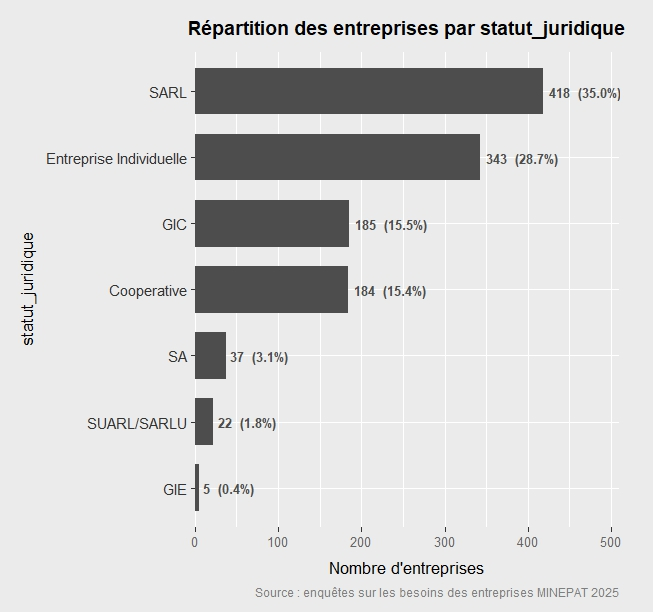
\includegraphics[width=0.75\textwidth]{statut.jpeg}
  \caption{Répartition des entreprises enquêtées par statut juridique}
  \label{fig:statut_juridique}
\end{figure}

\subsubsection{Répartition des entreprises par région}

Plus de la moitié des entreprises interrogées sont implantées dans les régions du Centre et du Littoral, avec respectivement 39,3\,\% et 17,8\,\%. Les régions du Nord-Ouest et du Sud-Ouest ferment la marche avec respectivement 2,7\,\% et 2,8\,\% des entreprises étudiées.

\begin{figure}[H]
  \centering
  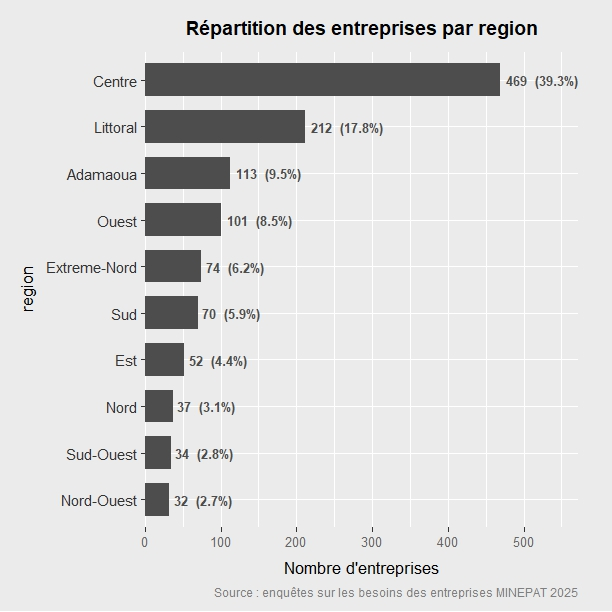
\includegraphics[width=0.75\textwidth]{repartition_region.jpeg}
  \caption{Répartition des entreprises enquêtées par région}
  \label{fig:region}
\end{figure}

\subsubsection{Répartition des entreprises par taille}

La distribution des entreprises par taille reflète la structure du tissu productif camerounais, caractérisé par une prédominance des petites entreprises et des très petites entreprises. Les grandes entreprises sont très peu nombreuses et constituent 1,3\,\% des entreprises interrogées.

\begin{figure}[H]
  \centering
  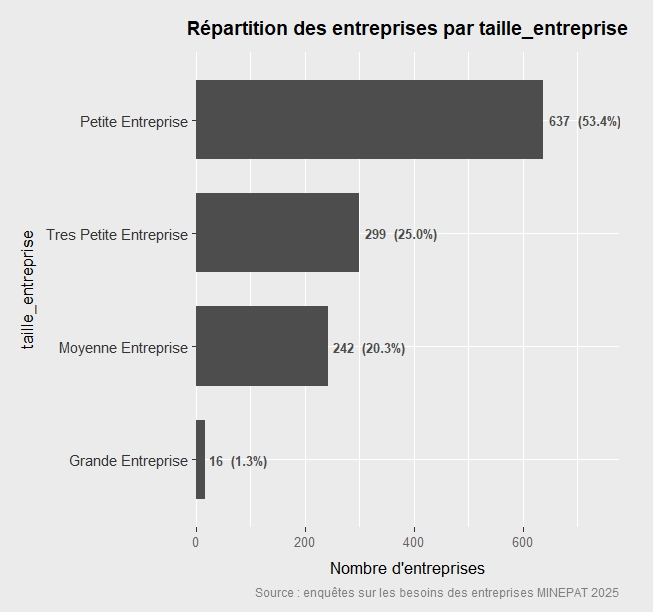
\includegraphics[width=0.75\textwidth]{repartition_taille.jpeg}
  \caption{Répartition des entreprises enquêtées par taille}
  \label{fig:taille}
\end{figure}

\subsubsection{Répartition des entreprises par ancienneté}

Ce sont les entreprises de 5 à 9 ans d'âge qui se sont le plus prêtées à l'enquête, avec 39,0\,\% de participation. Les entreprises n'ayant pas plus de 4 ans sont relativement nombreuses avec un pourcentage de 31,2\,\%.

\begin{figure}[H]
  \centering
  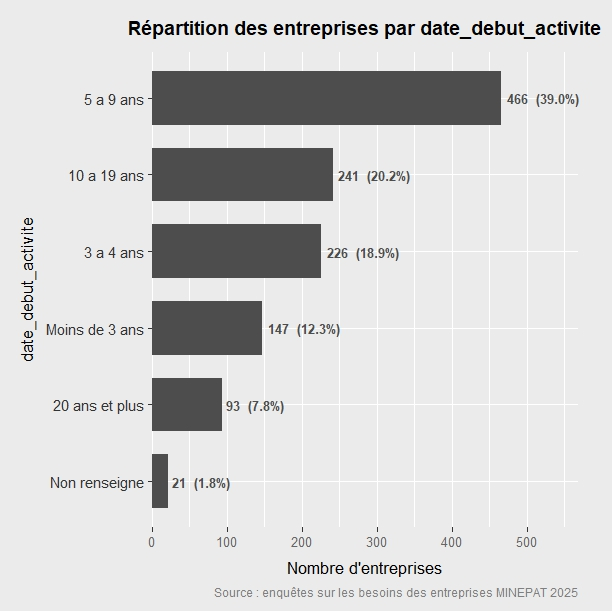
\includegraphics[width=0.75\textwidth]{anciennete.jpeg}
  \caption{Répartition des entreprises enquêtées par ancienneté}
  \label{fig:anciennete}
\end{figure}

\subsubsection{Répartition des entreprises par secteur d'activité}

Le secteur de l'agriculture et de l'agroalimentaire est le plus représenté, détenant à lui seul 62,6\,\% des entreprises étudiées. Les secteurs de l'industrie manufacturière et des Technologies de l'Information et de la Communication sont assez peu nombreux, avec respectivement 5,2\,\% et 3,7\,\%.

\begin{figure}[H]
  \centering
  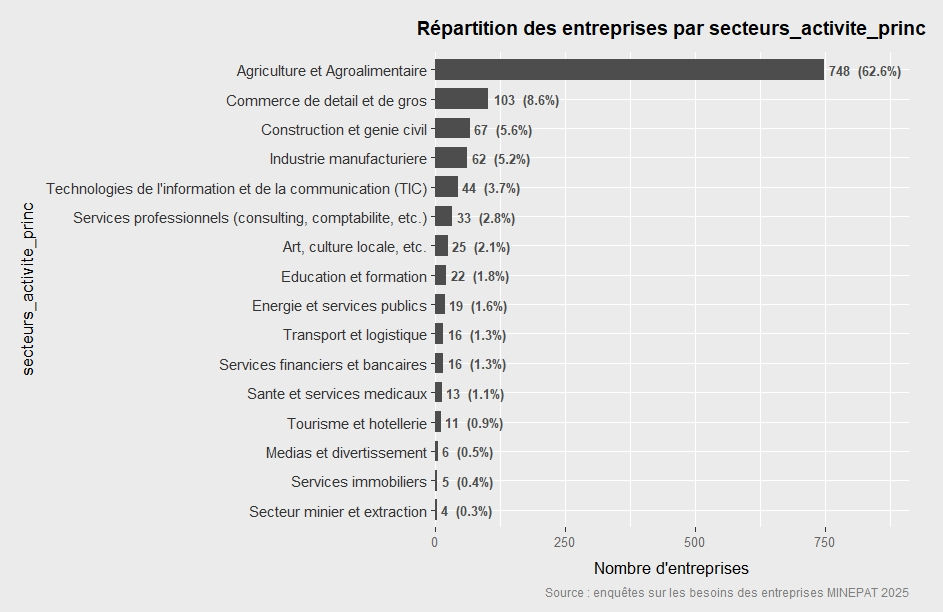
\includegraphics[width=0.75\textwidth]{repartition_activite.jpeg}
  \caption{Répartition des entreprises enquêtées par secteur d'activité}
  \label{fig:secteur}
\end{figure}

\subsubsection{Répartition des besoins exprimés}

Le besoin qui revient le plus est celui du financement avec un taux de 20,1\,\%. Ce résultat s'explique par la prédominance des \gls{tpe} et des \gls{pme} qui ont besoin de fonds pour une meilleure implantation. Le besoin en équipements arrive en deuxième position avec 19,4\,\%. Le besoin en transport est le moins fréquent, ce qui traduirait l'existence d'infrastructures adéquates pour l'acheminement des produits dans les zones d'enquête.

\begin{figure}[H]
  \centering
  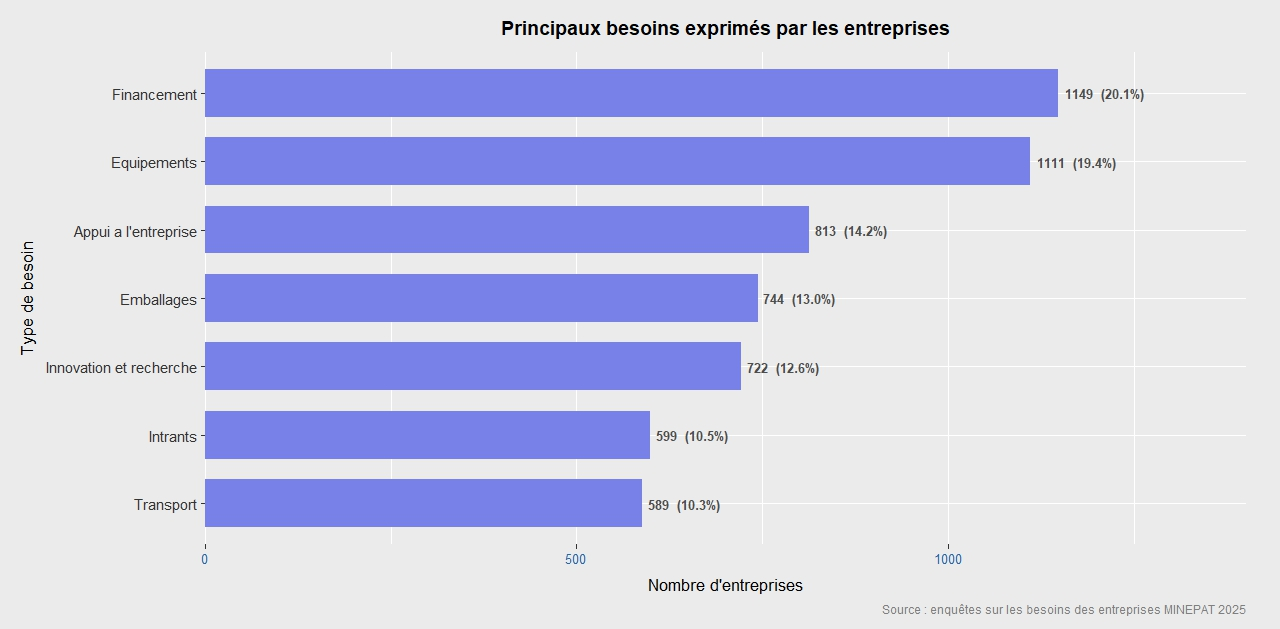
\includegraphics[width=0.75\textwidth]{repartition_besoins.jpeg}
  \caption{Répartition globale des besoins exprimés par les entreprises enquêtées}
  \label{fig:besoins_global}
\end{figure}

%-------------------------------------------------------------
\subsection{Résultats de l'analyse bivariée}
\label{subsec:bivariee}
%-------------------------------------------------------------

L'analyse bivariée a consisté à croiser les variables descriptives des entreprises avec les besoins qu'elles ont exprimés, afin d'identifier d'éventuelles associations structurelles. Deux outils ont été mobilisés : les tableaux de contingence et le test du $\chi^2$ de Pearson accompagné du coefficient $V$ de Cramér \cite{saporta2010}.

\subsubsection{Répartition des besoins selon le statut juridique}

\begin{figure}[H]
  \centering
  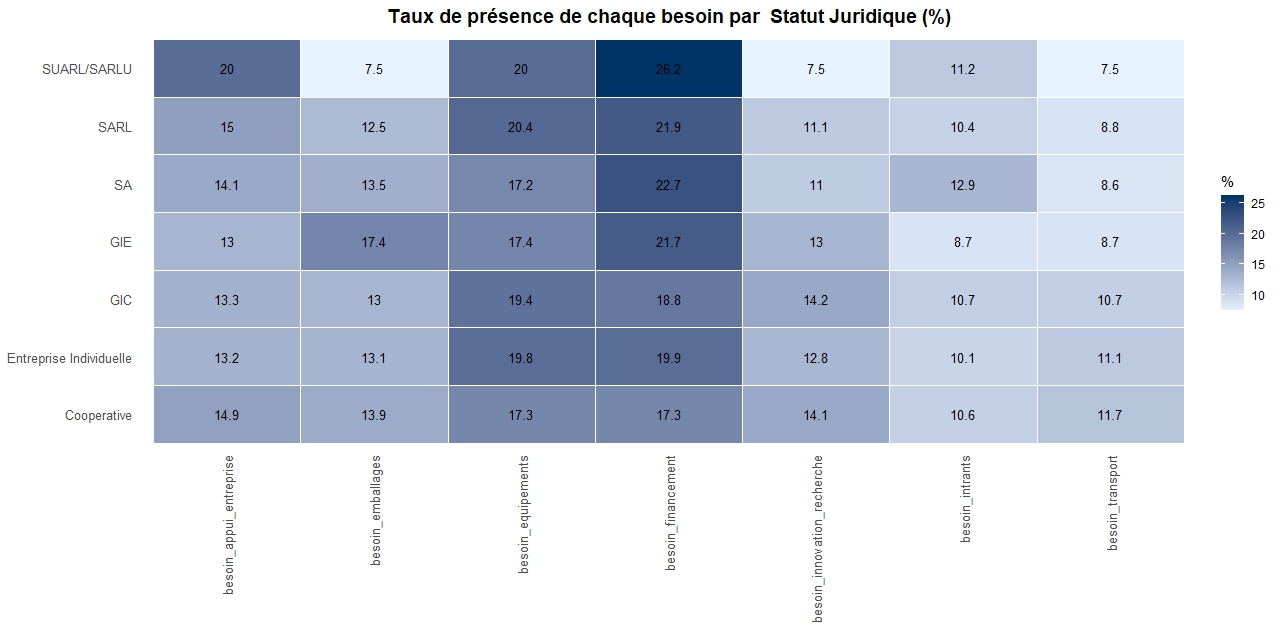
\includegraphics[width=\textwidth]{carte_chaleur_besoins_statut_juridique.jpeg}
  \caption{Distribution des besoins des entreprises selon le statut juridique}
  \label{fig:besoins_statut}
\end{figure}

\begin{table}[H]
  \centering
  \caption{Test du $\chi^2$ entre le statut juridique et les besoins des entreprises}
  \label{tab:khi2_statut}
  \renewcommand{\arraystretch}{1.4}
  \begin{tabularx}{\textwidth}{>{\raggedright\arraybackslash}X r r >{\centering\arraybackslash}p{2.8cm} r}
    \toprule
    \rowcolor{primary!15}
    \textbf{Besoin} & \textbf{$\chi^2$} & \textbf{p-valeur} & \textbf{Significatif} & \textbf{$V$ Cramér} \\
    \midrule
    Besoin en intrants        & 14,26 & 0,027  & Oui ($p < 0{,}05$) & 0,109 \\
    \rowcolor{lightgray}
    Besoin en financement     &  2,94 & 0,817  & Non                & 0,050 \\
    Besoin en emballages      & 44,47 & $<0{,}001$ & Oui ($p < 0{,}05$) & 0,193 \\
    \rowcolor{lightgray}
    Besoin en transport       & 50,44 & $<0{,}001$ & Oui ($p < 0{,}05$) & 0,206 \\
    Appui aux entreprises     & 26,32 & $<0{,}001$ & Oui ($p < 0{,}05$) & 0,148 \\
    \rowcolor{lightgray}
    Besoin en équipements     & 61,66 & $<0{,}001$ & Oui ($p < 0{,}05$) & 0,227 \\
    Innovation et recherche   & 77,88 & $<0{,}001$ & Oui ($p < 0{,}05$) & 0,255 \\
    \bottomrule
  \end{tabularx}
\end{table}

Les résultats révèlent que le statut juridique est significativement associé à six des sept besoins étudiés, à l'exception du besoin en financement ($\chi^2 = 2{,}94$ ; $p = 0{,}817$). Ce dernier constitue une exception notable : il est exprimé de manière relativement homogène quelle que soit la forme juridique de l'entreprise, suggérant que la contrainte financière est une réalité transversale à l'ensemble du tissu économique.

\subsubsection{Répartition des besoins selon la région}

\begin{figure}[H]
  \centering
  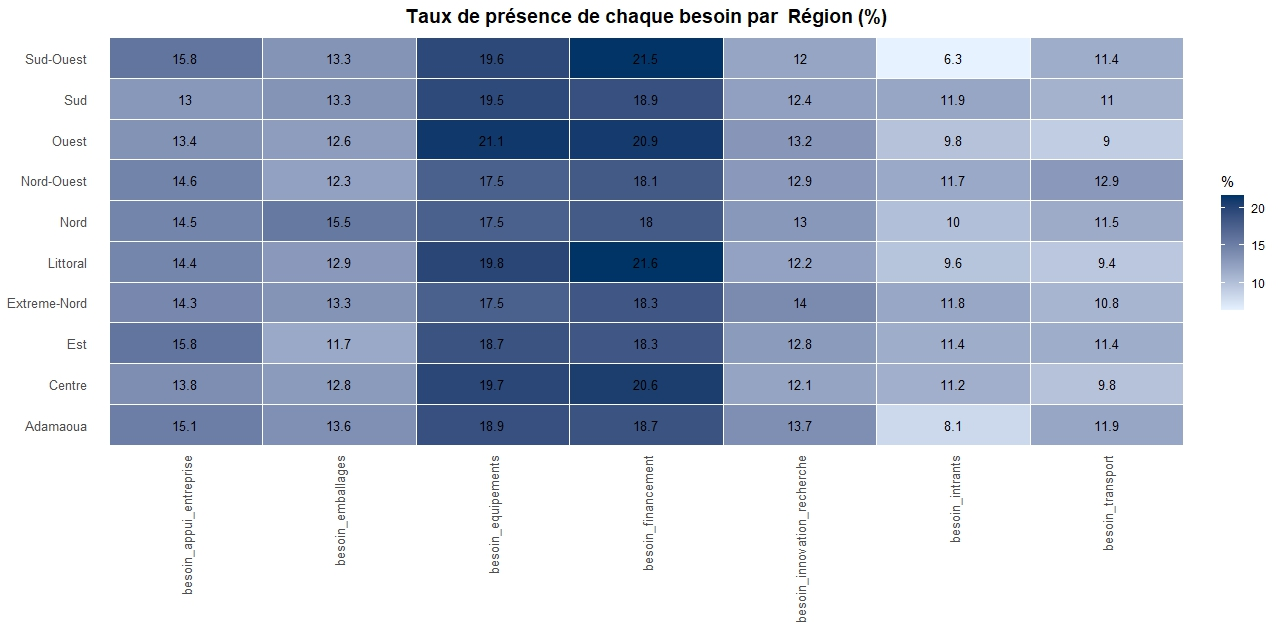
\includegraphics[width=\textwidth]{carte_chaleur_besoins_region.jpeg}
  \caption{Distribution des besoins des entreprises selon la région d'implantation}
  \label{fig:besoins_region}
\end{figure}

\begin{table}[H]
  \centering
  \caption{Test du $\chi^2$ entre la région d'implantation et les besoins des entreprises}
  \label{tab:khi2_region}
  \renewcommand{\arraystretch}{1.4}
  \begin{tabularx}{\textwidth}{>{\raggedright\arraybackslash}X r r >{\centering\arraybackslash}p{2.8cm} r}
    \toprule
    \rowcolor{primary!15}
    \textbf{Besoin} & \textbf{$\chi^2$} & \textbf{p-valeur} & \textbf{Significatif} & \textbf{$V$ Cramér} \\
    \midrule
    Besoin en intrants        & 28,91 & $<0{,}001$ & Oui ($p < 0{,}05$) & 0,156 \\
    \rowcolor{lightgray}
    Besoin en financement     &  6,21 & 0,718  & Non                & 0,072 \\
    Besoin en emballages      & 18,69 & 0,028  & Oui ($p < 0{,}05$) & 0,125 \\
    \rowcolor{lightgray}
    Besoin en transport       & 29,83 & $<0{,}001$ & Oui ($p < 0{,}05$) & 0,158 \\
    Appui aux entreprises     & 23,36 & 0,005  & Oui ($p < 0{,}05$) & 0,140 \\
    \rowcolor{lightgray}
    Besoin en équipements     & 28,25 & $<0{,}001$ & Oui ($p < 0{,}05$) & 0,154 \\
    Innovation et recherche   & 23,77 & 0,005  & Oui ($p < 0{,}05$) & 0,141 \\
    \bottomrule
  \end{tabularx}
\end{table}

La région d'implantation est significativement associée à six besoins sur sept, le besoin en financement étant à nouveau le seul sans association significative. Les besoins en transport ($V = 0{,}158$) et en intrants ($V = 0{,}156$) présentent les associations les plus fortes, ce qui est cohérent avec les disparités infrastructurelles importantes entre les régions camerounaises.

\subsubsection{Répartition des besoins selon l'ancienneté}

\begin{table}[H]
  \centering
  \caption{Test du $\chi^2$ entre l'ancienneté et les besoins des entreprises}
  \label{tab:khi2_anciennete}
  \renewcommand{\arraystretch}{1.4}
  \begin{tabularx}{\textwidth}{>{\raggedright\arraybackslash}X r r >{\centering\arraybackslash}p{2.8cm} r}
    \toprule
    \rowcolor{primary!15}
    \textbf{Besoin} & \textbf{$\chi^2$} & \textbf{p-valeur} & \textbf{Significatif} & \textbf{$V$ Cramér} \\
    \midrule
    Besoin en intrants        &  6,46 & 0,264  & Non  & 0,074 \\
    \rowcolor{lightgray}
    Besoin en financement     &  4,44 & 0,488  & Non  & 0,061 \\
    Besoin en emballages      &  5,09 & 0,405  & Non  & 0,065 \\
    \rowcolor{lightgray}
    Besoin en transport       &  5,52 & 0,356  & Non  & 0,068 \\
    Appui aux entreprises     & 11,84 & 0,037  & Oui ($p < 0{,}05$) & 0,100 \\
    \rowcolor{lightgray}
    Besoin en équipements     & 14,84 & 0,011  & Oui ($p < 0{,}05$) & 0,111 \\
    Innovation et recherche   & 20,10 & 0,001  & Oui ($p < 0{,}05$) & 0,130 \\
    \bottomrule
  \end{tabularx}
\end{table}

L'ancienneté est le critère présentant le moins d'associations significatives avec les besoins. Les entreprises jeunes (moins de 3 ans) expriment davantage de besoins en financement et en équipements. À l'inverse, les entreprises plus matures (20 ans et plus) expriment un besoin en innovation et en recherche plus marqué (13,9\,\%), témoignant d'une préoccupation croissante pour la compétitivité à long terme.

\subsubsection{Répartition des besoins selon le secteur d'activité}

\begin{table}[H]
  \centering
  \caption{Test du $\chi^2$ entre le secteur d'activité et les besoins des entreprises}
  \label{tab:khi2_secteur}
  \renewcommand{\arraystretch}{1.4}
  \begin{tabularx}{\textwidth}{>{\raggedright\arraybackslash}X r r >{\centering\arraybackslash}p{2.8cm} r}
    \toprule
    \rowcolor{primary!15}
    \textbf{Besoin} & \textbf{$\chi^2$} & \textbf{p-valeur} & \textbf{Significatif} & \textbf{$V$ Cramér} \\
    \midrule
    Besoin en intrants        & 103,48 & $<0{,}001$ & Oui ($p < 0{,}05$) & 0,294 \\
    \rowcolor{lightgray}
    Besoin en financement     &  34,10 & 0,003  & Oui ($p < 0{,}05$) & 0,169 \\
    Besoin en emballages      & 306,81 & $<0{,}001$ & Oui ($p < 0{,}05$) & 0,507 \\
    \rowcolor{lightgray}
    Besoin en transport       & 147,87 & $<0{,}001$ & Oui ($p < 0{,}05$) & 0,352 \\
    Appui aux entreprises     &  20,13 & 0,167  & Non                & 0,130 \\
    \rowcolor{lightgray}
    Besoin en équipements     & 239,10 & $<0{,}001$ & Oui ($p < 0{,}05$) & 0,447 \\
    Innovation et recherche   & 163,49 & $<0{,}001$ & Oui ($p < 0{,}05$) & 0,370 \\
    \bottomrule
  \end{tabularx}
\end{table}

Le secteur d'activité constitue la variable présentant les associations les plus fortes avec les besoins : six besoins sur sept lui sont significativement liés, avec des valeurs de $V$ de Cramér particulièrement élevées pour le besoin en emballages ($V = 0{,}507$) et en équipements ($V = 0{,}447$). Ces résultats confirment que le secteur d'activité est le principal déterminant de la nature des besoins exprimés par les entreprises.

%-------------------------------------------------------------
\subsection{Résultats de l'analyse multidimensionnelle}
\label{subsec:multi}
%-------------------------------------------------------------

\subsubsection{Analyse des Correspondances Multiples (ACM)}

L'\gls{acm} a été conduite à l'aide du package \texttt{FactoMineR} du langage R \cite{lebart1994}, sur l'ensemble des variables qualitatives retenues.

\paragraph{Valeurs propres et inertie expliquée}

\begin{figure}[H]
  \centering
  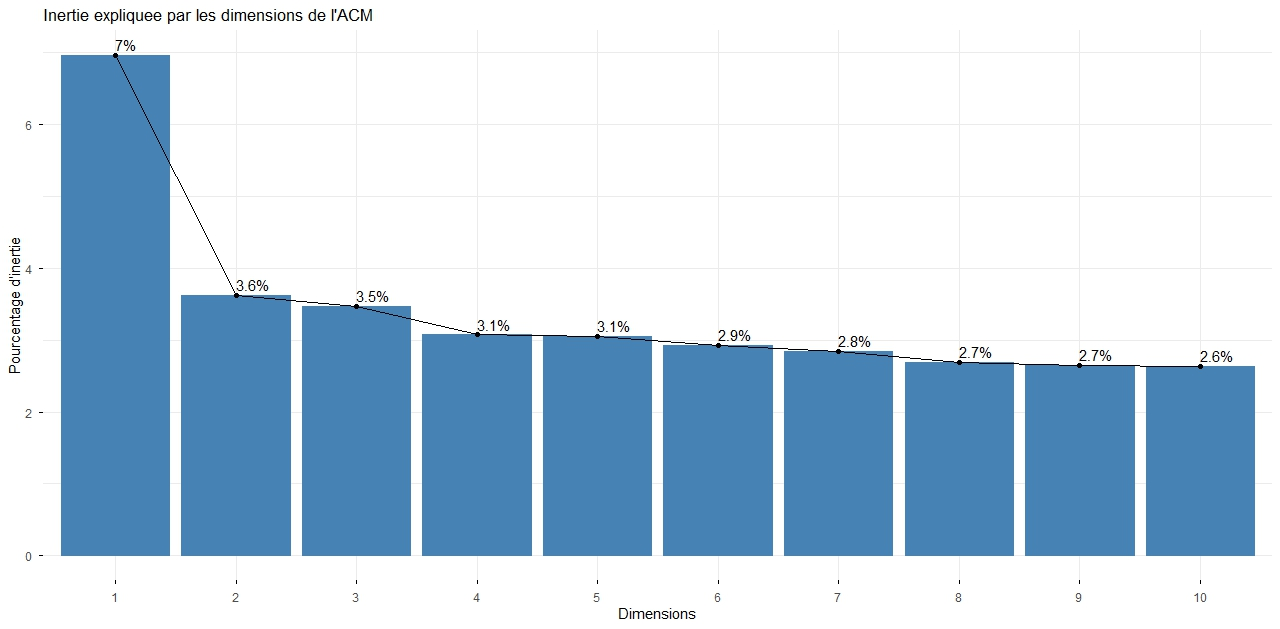
\includegraphics[width=0.75\textwidth]{contributionValeursPropres.jpeg}
  \caption{Éboulis des valeurs propres de l'ACM --- part d'inertie expliquée par axe factoriel}
  \label{fig:acm_vp}
\end{figure}

En application du critère du coude, les cinq premiers axes factoriels ont été retenus. Le premier axe capte 7\,\% de l'inertie totale et est fortement construit par les modalités liées aux besoins opérationnels et techniques (\texttt{besoin\_emballages\_Non}, \texttt{besoin\_innovation\_Non}, \texttt{besoin\_equipements\_Non}). Le second axe (3,6\,\%) est défini par des variables institutionnelles et géographiques (taille Moyenne Entreprise, forme juridique SA, région Ouest).

\paragraph{Projection des modalités sur le premier plan factoriel}

\begin{figure}[H]
  \centering
  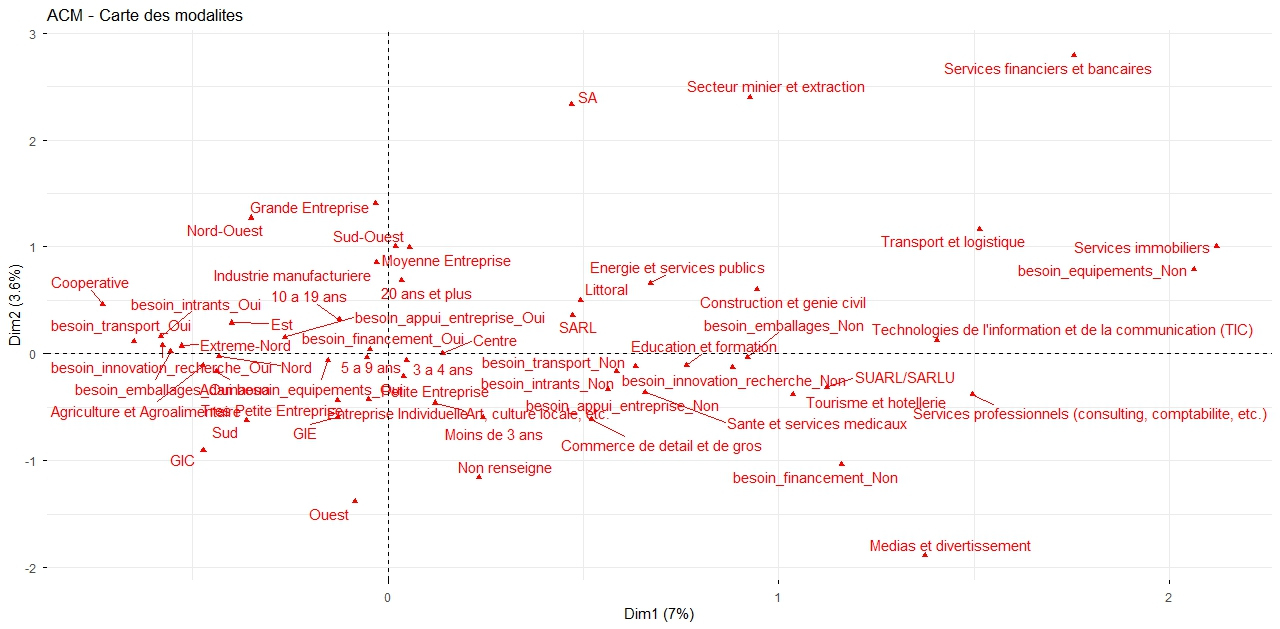
\includegraphics[width=\textwidth]{projectionDesCategories.jpeg}
  \caption{Projection des modalités sur le premier plan factoriel de l'ACM (axes 1 et 2)}
  \label{fig:acm_projection}
\end{figure}

L'axe 1 oppose les entreprises tertiaires des entreprises du secteur primaire à travers la présence ou l'absence de certains besoins. On observe la présence quasi au centre du besoin en financement, confirmant son caractère transversal.

\subsubsection{Classification Ascendante Hiérarchique (CAH)}

\begin{figure}[H]
  \centering
  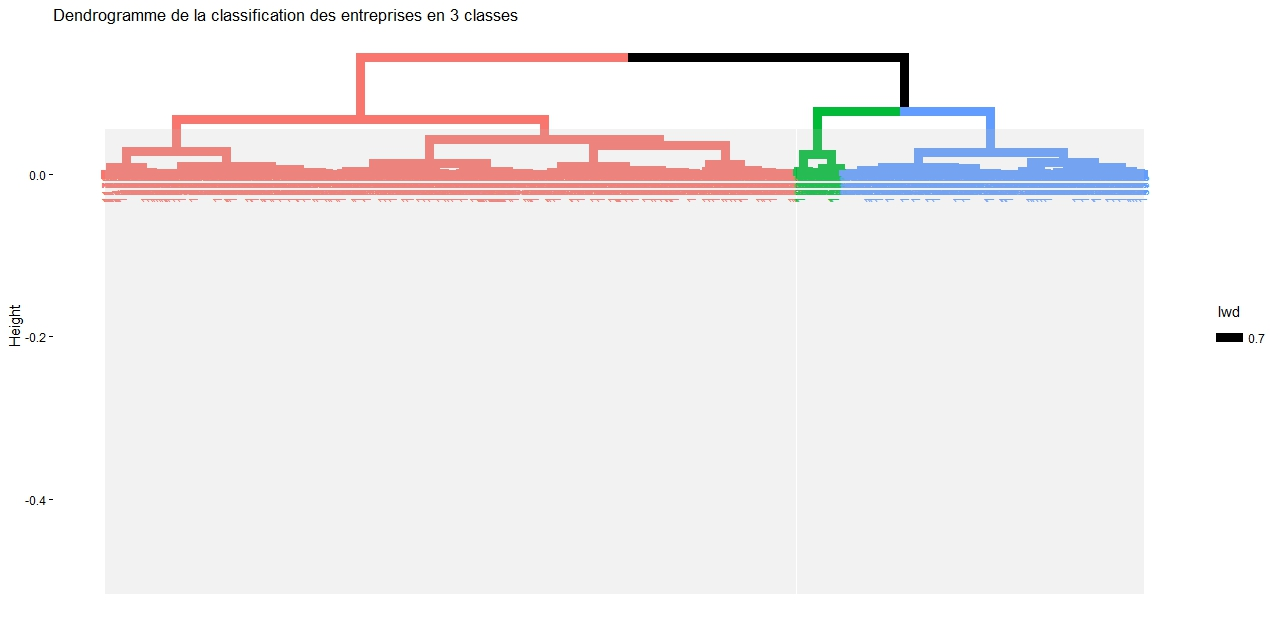
\includegraphics[width=0.85\textwidth]{dendrogramme.jpeg}
  \caption{Dendrogramme de la Classification Ascendante Hiérarchique (méthode de Ward)}
  \label{fig:dendrogramme}
\end{figure}

L'examen du dendrogramme révèle un saut d'inertie particulièrement marqué au passage de trois à deux classes, plaidant en faveur d'une \textbf{partition en trois classes}. Cette partition offre une granularité suffisante pour identifier des profils distincts et opérationnellement utiles.

\begin{figure}[H]
  \centering
  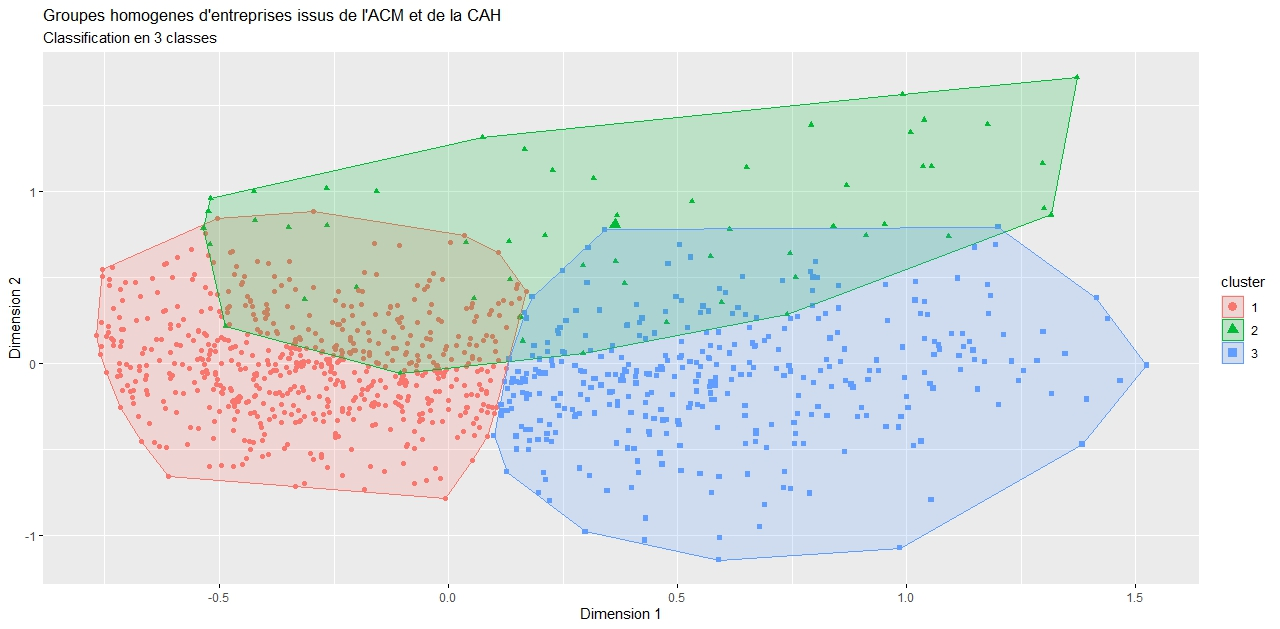
\includegraphics[width=\textwidth]{CAH.jpeg}
  \caption{Projection des trois classes obtenues par CAH sur le premier plan factoriel de l'ACM}
  \label{fig:cah_classes}
\end{figure}

Les trois classes sont caractérisées comme suit :

\begin{itemize}
  \item \textbf{Classe 1} --- [753 entreprises, 63,1\,\%] : profil dominant agricole et agroalimentaire. 81,1\,\% évoluent dans ce secteur, 52,5\,\% sont des petites entreprises, 36,3\,\% sont implantées dans la région du Centre~;

  \item \textbf{Classe 2} --- [57 entreprises, 4,8\,\%] : profil de services formalisés. 54,4\,\% sont des moyennes entreprises, 24,6\,\% offrent des services financiers et bancaires, 26,4\,\% ont plus de 20 ans d'ancienneté~;

  \item \textbf{Classe 3} --- [384 entreprises, 32,2\,\%] : profil intermédiaire diversifié. 31,2\,\% sont dans le secteur agricole, 59,6\,\% sont des petites entreprises, 45,6\,\% sont implantées dans la région du Centre.
\end{itemize}

\subsubsection{Analyse Factorielle Discriminante (AFD)}

\begin{figure}[H]
  \centering
  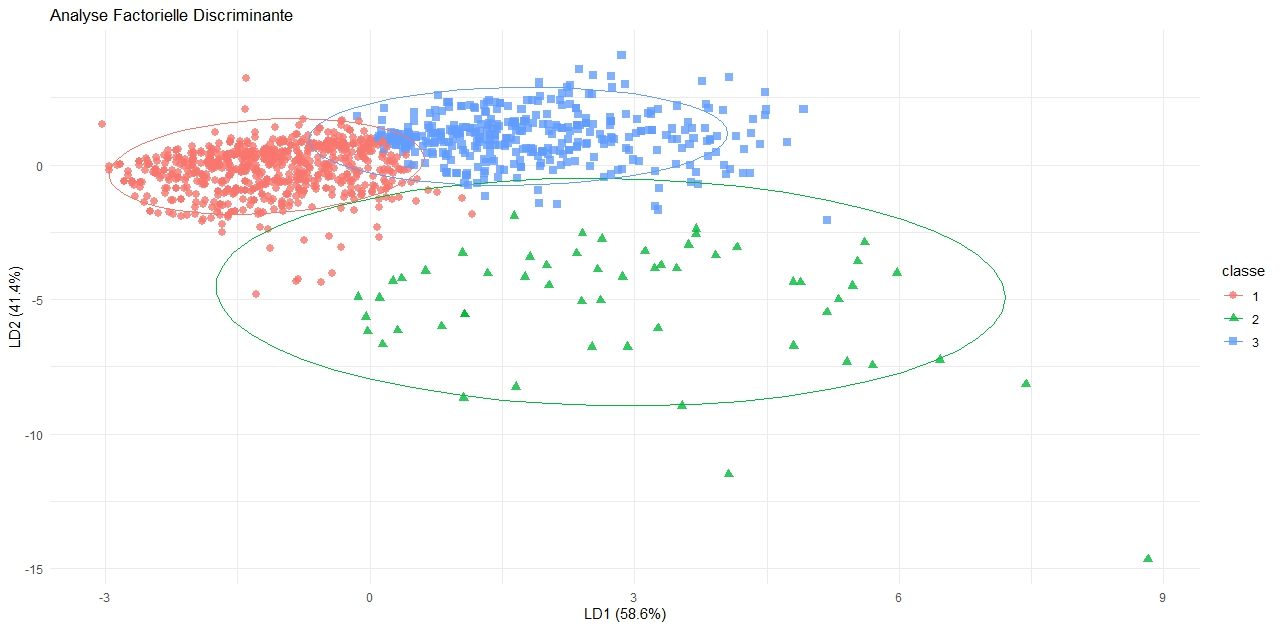
\includegraphics[width=0.85\textwidth]{AFDProjectionDesObservations.jpeg}
  \caption{Projection des entreprises et des centres de classes sur les axes discriminants de l'AFD}
  \label{fig:afd_projection}
\end{figure}

Les deux axes discriminants captent ensemble 100\,\% du pouvoir de séparation (LD1 : 58,6\,\% ; LD2 : 41,4\,\%). Les ellipses de confiance à 95\,\% confirment la pertinence statistique du modèle.

\begin{table}[H]
  \centering
  \caption{Indicateurs de performance du modèle discriminant}
  \label{tab:scores_modele}
  \renewcommand{\arraystretch}{1.4}
  \begin{tabularx}{\textwidth}{>{\raggedright\arraybackslash}X >{\centering\arraybackslash}p{3.5cm} >{\centering\arraybackslash}p{3cm}}
    \toprule
    \rowcolor{primary!15}
    \textbf{Indicateur} & \textbf{Valeur} & \textbf{Interprétation} \\
    \midrule
    Accuracy & 0,9724 & Excellent \\
    \rowcolor{lightgray}
    Kappa de Cohen & 0,9435 & Accord quasi-parfait \\
    Accuracy Lower (IC 95\,\%) & 0,9614 & --- \\
    \rowcolor{lightgray}
    Accuracy Upper (IC 95\,\%) & 0,9809 & --- \\
    Accuracy Null & 0,6307 & Seuil classifieur naïf \\
    \rowcolor{lightgray}
    Accuracy P-value & $5{,}16 \times 10^{-183}$ & Hautement significatif \\
    McNemar P-value & $8{,}50 \times 10^{-7}$ & Significatif ($p < 0{,}05$) \\
    \bottomrule
  \end{tabularx}
\end{table}

Le modèle affiche une précision globale de \textbf{97,24\,\%}, avec un Kappa de Cohen de \textbf{0,9435} (accord quasi-parfait). Le gain de performance par rapport au classifieur naïf est de $+34{,}17$ points de pourcentage, illustrant l'apport réel du modèle discriminant.

%-------------------------------------------------------------
\section{Présentation de la plateforme Business Partnership}
\label{sec:plateforme}
%-------------------------------------------------------------

\subsection{Prérequis et environnement d'exécution}

La plateforme \textit{Business Partnership} a été développée sous Python 3.11 et Django 4.2, avec SQLite3 comme système de gestion de base de données en environnement de développement. Elle est accessible via un navigateur web standard. L'accès à la plateforme nécessite un compte utilisateur valide, créé lors de la phase d'inscription.

\subsection{Flux d'inscription et d'onboarding}

\subsubsection{Page d'accueil et inscription}

La page d'accueil de la plateforme présente le contexte institutionnel du projet et invite l'utilisateur à créer un compte. Le formulaire d'inscription collecte les informations d'identification de base (nom d'utilisateur, adresse électronique, mot de passe).

\begin{figure}[H]
  \centering
  % \includegraphics[width=0.85\textwidth]{page_accueil.png}
  \begin{tikzpicture}
    \node[draw=primary, fill=primary!5, rounded corners=5pt,
      minimum width=12cm, minimum height=5cm, align=center] {
      \textbf{\large\color{primary} Business Partnership}\\[8pt]
      \textcolor{darkgray}{\small Plateforme gouvernementale de cartographie et de mise en relation}\\[12pt]
      \fbox{\parbox{5cm}{\centering\small\textbf{Créer un compte}\\[4pt]
        Nom d'utilisateur : \underline{\hspace{3cm}}\\[3pt]
        Email : \underline{\hspace{3cm}}\\[3pt]
        Mot de passe : \underline{\hspace{3cm}}\\[6pt]
        \textcolor{primary}{\textbf{[S'inscrire]}}}}
    };
  \end{tikzpicture}
  \caption{Maquette de la page d'accueil et du formulaire d'inscription de la plateforme}
  \label{fig:page_accueil}
\end{figure}

\subsubsection{Formulaire de profil d'entreprise}

Après la création du compte, l'utilisateur est redirigé vers le formulaire de profil de l'entreprise, où il renseigne les caractéristiques qui seront utilisées par le pipeline de classification. Les champs sont alimentés dynamiquement depuis la base de données (listes déroulantes pour la région, la taille, le secteur, le statut juridique et l'ancienneté).

\subsubsection{Formulaire de besoins}

Le formulaire de besoins (\texttt{BesoinsForm}) présente les sept catégories de besoins sous forme de cases à cocher. Chaque réponse binaire (Oui/Non) est enregistrée dans le modèle \texttt{CustomUser} et transmise au pipeline de classification.

\begin{figure}[H]
  \centering
  \begin{tikzpicture}
    \node[draw=secondary, fill=secondary!5, rounded corners=5pt,
      minimum width=12cm, minimum height=5.5cm, align=left, inner sep=12pt] {
      \textbf{\color{primary} Étape 3 : Vos besoins}\\[6pt]
      \small
      $\square$ Besoin en intrants (matières premières, semences, intrants agricoles)\\[3pt]
      $\boxtimes$ Besoin en financement (crédit, investissement, subvention)\\[3pt]
      $\square$ Besoin en emballages (conditionnement, packaging)\\[3pt]
      $\boxtimes$ Besoin en transport (logistique, acheminement)\\[3pt]
      $\square$ Besoin en appui aux entreprises (conseil, accompagnement)\\[3pt]
      $\boxtimes$ Besoin en équipements (machines, outils de production)\\[3pt]
      $\square$ Besoin en innovation et recherche (nouvelles technologies)\\[8pt]
      \textcolor{primary}{\textbf{[Suivant →]}}
    };
  \end{tikzpicture}
  \caption{Maquette du formulaire de besoins (Étape 3 du flux d'onboarding)}
  \label{fig:formulaire_besoins}
\end{figure}

\subsection{Page de recommandations}

Après la classification automatique, l'entreprise est redirigée vers sa page de recommandations. Cette page affiche :

\begin{itemize}
  \item Le \textbf{profil de la classe d'appartenance} : libellé et description de la classe issue de la \gls{cah}~;
  \item Le \textbf{récapitulatif des besoins} déclarés, sous forme de badges colorés~;
  \item La \textbf{liste des partenaires potentiels}, c'est-à-dire les entreprises enregistrées sur la plateforme ayant déclaré pouvoir répondre aux besoins de la classe d'appartenance, classées par pertinence~;
  \item Des \textbf{filtres interactifs} permettant de cibler les recommandations par région, secteur d'activité ou taille d'entreprise.
\end{itemize}

\begin{figure}[H]
	\centering
	\begin{tikzpicture}
		\node[draw=primary, fill=primary!5, rounded corners=5pt,
		minimum width=12cm, minimum height=7cm, align=left, inner sep=12pt] {
			\textbf{\large\color{primary} Tableau de bord --- Business Partnership}\\[6pt]
			\textbf{Votre classe :} \colorbox{primary!20}{\textcolor{primary}{\textbf{Classe 1 --- Profil Agricole et Agroalimentaire}}}\\[6pt]
			\textbf{Vos besoins :}
			\colorbox{accent!20}{\small Financement} \quad
			\colorbox{accent!20}{\small Transport} \quad
			\colorbox{accent!20}{\small Équipements}\\[10pt]
			\noindent\rule{11.1cm}{0.5pt}\\[8pt]
			\textbf{Partenaires recommandés :}\\[4pt]
			\small
			\fbox{\parbox{10cm}{\textbf{AgriEquip Sarl} --- Secteur : Équipements agricoles --- Région : Centre\\
					\textcolor{secondary}{$\checkmark$ Peut répondre à vos besoins en équipements et financement}}}\\[4pt]
			\fbox{\parbox{10cm}{\textbf{CamTransport SA} --- Secteur : Logistique --- Région : Littoral\\
					\textcolor{secondary}{$\checkmark$ Peut répondre à vos besoins en transport}}}\\[8pt]
			\textcolor{darkgray}{\small Filtres : \underline{Région} \quad \underline{Secteur} \quad \underline{Taille}}
		};
	\end{tikzpicture}
	\caption{Maquette de la page de recommandations de la plateforme Business Partnership}
	\label{fig:page_recommandations}
\end{figure}

\subsection{Interface d'administration}

La plateforme intègre l'interface d'administration native de Django, permettant aux agents du \gls{minepat} de :

\begin{itemize}
  \item Gérer les comptes entreprises (création, modification, désactivation)~;
  \item Consulter et exporter la liste des entreprises enregistrées avec leurs caractéristiques~;
  \item Mettre à jour les données de référence (régions, secteurs, classes, capacités de réponse)~;
  \item Superviser les statistiques d'utilisation de la plateforme.
\end{itemize}

\subsection{Limites du travail}

Plusieurs limites doivent être mentionnées. Premièrement, la base d'entraînement des modèles statistiques est constituée de 1~194 entreprises, ce qui constitue un échantillon de taille modérée au regard de la diversité du tissu économique camerounais. Une mise à jour régulière des modèles sera nécessaire au fur et à mesure que de nouvelles entreprises s'inscriront sur la plateforme. Deuxièmement, la plateforme est actuellement en environnement de développement (SQLite3) et nécessite une migration vers PostgreSQL et un déploiement sur un serveur institutionnel pour une mise en production. Troisièmement, les données géographiques (coordonnées GPS des entreprises) ne sont pas encore intégrées, limitant la fonctionnalité de cartographie visuelle.

\subsection{Perspectives}

Plusieurs axes d'amélioration sont identifiés pour les versions futures de la plateforme :

\begin{itemize}
  \item \textbf{Intégration d'une cartographie interactive} : en s'appuyant sur les coordonnées géographiques des entreprises, un module de cartographie basé sur Leaflet.js ou OpenStreetMap permettrait une visualisation géographique des besoins et des partenaires~;

  \item \textbf{Réentraînement automatique des modèles} : la mise en place d'un pipeline de réentraînement périodique des modèles statistiques, déclenché lors de l'atteinte d'un seuil d'inscriptions, permettrait de maintenir la pertinence des recommandations~;

  \item \textbf{Module de messagerie institutionnelle} : l'ajout d'un système de messagerie sécurisée permettant aux entreprises recommandées d'entrer directement en contact constituerait la prochaine étape logique dans la création effective de partenariats~;

  \item \textbf{Tableau de bord analytique pour le MINEPAT} : un tableau de bord d'aide à la décision destiné aux agents de la \gls{dape}, affichant en temps réel les statistiques d'inscription et les tendances des besoins, permettrait d'alimenter directement les rapports de conjoncture économique.
\end{itemize}

%============================================================
%  CONCLUSION GÉNÉRALE
%============================================================
\chapter*{Conclusion Générale}
\addcontentsline{toc}{chapter}{Conclusion Générale}
\markboth{Conclusion Générale}{Conclusion Générale}

Ce travail a répondu à un double objectif : proposer une cartographie statistique rigoureuse des besoins des entreprises du tissu productif camerounais, et concevoir une plateforme numérique gouvernementale permettant de mettre en relation ces entreprises sur la base de leurs profils et besoins respectifs.

Sur le plan statistique, l'analyse de 1~194 entreprises à travers un pipeline ACM-CAH-AFD a permis d'identifier trois profils distincts d'entreprises camerounaises, reflétant la structure duale du tissu économique national : un large groupe dominé par les activités agricoles et agroalimentaires, un groupe restreint de services formalisés et financiers, et un groupe intermédiaire diversifié. Les résultats révèlent que le financement est un besoin universel, transversal à toutes les classes, tandis que les besoins en équipements, emballages et transport sont fortement déterminés par le secteur d'activité. Le modèle discriminant obtenu affiche une précision de 97,24\,\% (Kappa~$= 0{,}94$), confirmant la robustesse de la classification.

Sur le plan technologique, la plateforme \textit{Business Partnership}, développée sous Django/Python, intègre un pipeline de classification automatique permettant d'affecter chaque entreprise à sa classe d'appartenance et de générer des recommandations personnalisées de partenaires potentiels. Elle constitue le premier outil institutionnel de ce type dans le paysage numérique camerounais, offrant un cadre formel, structuré et étendu pour la mise en relation des entreprises locales.

Au-delà des résultats produits, ce travail illustre la complémentarité entre les méthodes de Data Science et les enjeux de politique économique publique. Il montre que les techniques d'analyse multivariée, habituellement mobilisées dans des contextes académiques, peuvent être directement opérationnalisées dans des outils au service des décideurs et des acteurs économiques.

\medskip

%============================================================
%  BIBLIOGRAPHIE
%============================================================
\printbibliography[heading=bibintoc, title={Bibliographie}]

%============================================================
%  ANNEXES
%============================================================
\appendix

\chapter{Questionnaire de l'enquête MINEPAT 2025}
\label{ann:questionnaire}

Le questionnaire de l'enquête a été structuré en deux grandes parties, conformément aux deux fichiers de données produits lors de la collecte. La première partie (correspondant au fichier \texttt{identifications.csv}) comprend les questions d'identification de l'entreprise : raison sociale, statut juridique, région, localisation, taille, date de début d'activité, secteur d'activité, branche d'activité, biens et services produits, coordonnées téléphoniques et électroniques. La seconde partie (correspondant au fichier \texttt{besoins.csv}) comprend les questions relatives aux besoins exprimés : type de besoin, détail du besoin et plateformes de mise en relation déjà utilisées.

\chapter{Code Python du module de classification}
\label{ann:code}

Le code complet du module \texttt{classifier.py} est présenté dans la section~\ref{lst:classifier} du chapitre~3. L'ensemble du code source de la plateforme est versionné sous Git et disponible sur le dépôt institutionnel de la \gls{dape}.

\chapter{Manuel d'utilisation de la plateforme}
\label{ann:manuel}

\section*{Prérequis techniques}

\begin{itemize}
  \item Python 3.11 ou supérieur~;
  \item Django 4.2~;
  \item Bibliothèques Python : Pandas, NumPy, Scikit-learn, Pickle~;
  \item Navigateur web moderne (Chrome, Firefox, Edge).
\end{itemize}

\section*{Installation}

\begin{lstlisting}[language=bash, caption={Procédure d'installation de la plateforme}]
# Cloner le dépôt
git clone https://github.com/minepat-dape/business-partnership.git
cd business-partnership

# Créer un environnement virtuel
python -m venv venv
source venv/bin/activate  # Linux/Mac
venv\Scripts\activate     # Windows

# Installer les dépendances
pip install -r requirements.txt

# Appliquer les migrations
python manage.py migrate

# Charger les données de référence
python manage.py loaddata initial_data.json

# Lancer le serveur de développement
python manage.py runserver
\end{lstlisting}

\section*{Accès à la plateforme}

Après démarrage du serveur, la plateforme est accessible à l'adresse \url{http://127.0.0.1:8000/}. L'interface d'administration est accessible à l'adresse \url{http://127.0.0.1:8000/admin/} après création d'un super-utilisateur via la commande \texttt{python manage.py createsuperuser}.

\end{document}
